\documentclass[xcolor=pdftex,table,10pt]{beamer}
\usepackage{pgfpages}
%\pgfpagesuselayout{4 on 1}[a4paper, border shrink=5mm, landscape]


\mode<presentation> {
  \usetheme{Madrid}
  \usecolortheme{seahorse}
  \usecolortheme{rose}
}

\AtBeginSection[]
{
  \begin{frame}<beamer>
    \frametitle{Outline}
    \tableofcontents[currentsection,hideothersubsections]
  \end{frame}
}

\AtBeginSubsection[]
{
  \begin{frame}<beamer>
    \frametitle{Outline}
    \tableofcontents[currentsection,currentsubsection]
  \end{frame}
}

%change bottom line
\setbeamertemplate{footline}
{
  \leavevmode%
  \hbox{%
  \begin{beamercolorbox}[wd=.23\paperwidth,ht=2.25ex,dp=1ex,center]{author in head/foot}%
    \usebeamerfont{author in head/foot}\insertshortauthor
  \end{beamercolorbox}%
  \begin{beamercolorbox}[wd=.54\paperwidth,ht=2.25ex,dp=1ex,center]{title in head/foot}%
    \usebeamerfont{title in head/foot}\insertshorttitle
  \end{beamercolorbox}%
  \begin{beamercolorbox}[wd=.23\paperwidth,ht=2.25ex,dp=1ex,right]{date in head/foot}%
    \usebeamerfont{date in head/foot}\insertshortdate{}\hspace*{2em}
    \insertframenumber{} / \inserttotalframenumber\hspace*{2ex} 
  \end{beamercolorbox}}%
  \vskip0pt%
}

\usepackage[english]{babel}
\usepackage[latin1]{inputenc}
\usepackage{times}
\usepackage{listings}
\usepackage{colortbl}
\usepackage{tikz}
\usepackage{verbatim}
\usepackage{algorithm}
\usepackage{algorithmic}
\usepackage{amsmath}
\usepackage{amsfonts}
\usepackage{url}
\usetikzlibrary{shapes,arrows,snakes,backgrounds}
\usefonttheme[onlymath]{serif}
%\usepackage[T1]{fontenc}
%\usepackage{color}
%\usepackage[x11names, rgb]{xcolor}
%\usepackage{dot2texi}
%\usepackage{pgfplots}
%\usefonttheme{professionalfonts}

\tikzstyle{format} = [draw, thin, fill=blue!20]
\tikzstyle{pblock} = [rectangle, draw, fill=blue!20, text width=6em, text centered, rounded corners, minimum height=0.4em]
\tikzstyle{mblock} = [rectangle, draw, fill=green!20, text width=6em, text centered, rounded corners, minimum height=0.4em]
\tikzstyle{bblock} = [rectangle, draw, fill=gray!20, text width=6em, text centered, rounded corners, minimum height=0.4em]
\tikzstyle{prblock} = [rectangle, draw, fill=red!20, text width=6em, text centered, rounded corners, minimum height=0.4em]
\tikzstyle{rblock} = [rectangle, draw, fill=black!50, text width=6em, text centered, rounded corners, minimum height=0.4em]
\tikzstyle{block} = [rectangle, draw, fill=gray!20, text centered, rounded corners]
\tikzstyle{decision} = [diamond, draw, fill=blue!20, text width=4.5em, text badly centered, node distance=3cm, inner sep=0pt]
\tikzstyle{medium} = [ellipse, draw, thin, fill=green!20, minimum height=2.5em]
\tikzstyle{cloud} = [draw, ellipse,fill=red!20, node distance=3cm, minimum height=2em]
\tikzstyle{line} = [draw, -latex']
\tikzstyle{emptyblock} = [rectangle]
\tikzstyle{progblock} = [rectangle, draw, fill=yellow!20, text width=6em, text centered, minimum height=0.4em]
\tikzstyle{null} = [rectangle, fill=blue!0, text width=6em, text centered, rounded corners, minimum height=0.4em]


\newcommand{\opal}{\textsc{OPAL }}
\renewcommand {\Re}{{\mathbb{R}}}
\setbeamertemplate{navigation symbols}{} 

\title[PMAA 2010]{A Fast Parallel Poisson Solver on Irregular Domains}
\author[Y. Ineichen]{Yves Ineichen$^{*,**}$ \\ Andreas Adelmann$^{**}$ \\ Peter Arbenz$^{*}$}
\institute{$^{*}$Federal Institute of Technology\\ Department of Computer Science\\ Universitaetsstrasse 6, CH-8092 Zuerich, Switzerland \\ \vspace{0.2cm} $^{**}$Paul Scherrer Institute \\ Accelerator Modelling and Advanced Simulations \\ CH-5234 Villigen, Switzerland}
\date{1st July 2010}
\titlegraphic{
	\begin{columns}
		\begin{column}{3cm}
			\includegraphics[width=2cm]{ethlogo} \\
		\end{column}
		\begin{column}{2cm}
			
\includegraphics[width=3cm]{psilogo} \\
		\end{column}
	\end{columns}
}

\begin{document}

% For every picture that defines or uses external nodes, you'll have to
% apply the 'remember picture' style. To avoid some typing, we'll apply
% the style to all pictures.
\tikzstyle{every picture}+=[remember picture]

% By default all math in TikZ nodes are set in inline mode. Change this to
% displaystyle so that we don't get small fractions.
\everymath{\displaystyle}

	\lstset{language=C++, basicstyle=\small}

	\begin{frame}
            \titlepage
	\end{frame}
	
	\begin{frame}
	  \frametitle{Outline}
	  \tableofcontents
	\end{frame}

	\section{Motivation}

    \begin{frame}
		\frametitle{Vlasov-Poisson formulation for particle evolution}

        \tikzstyle{na} = [baseline=-.5ex]

		\begin{center}
		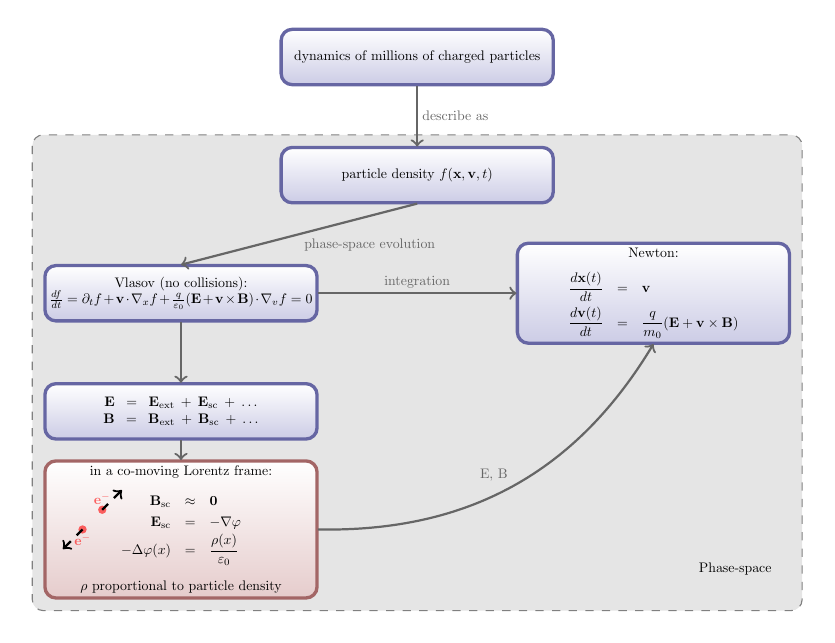
\begin{tikzpicture}[scale=0.5, transform shape, node distance = 3.0cm, auto]
			\tikzstyle{block} = [rectangle, draw, fill=blue!20, text width=19em, text centered, rounded corners, minimum height=4em, shade,top color=white,bottom color=blue!50!black!20, draw=blue!40!black!60, very thick]
			\tikzstyle{ablock} = [rectangle, draw, fill=red!20, text width=19em, text centered, rounded corners, minimum height=4em, shade,top color=white,bottom color=red!50!black!20, draw=red!40!black!60, very thick]
			\tikzstyle{line} = [draw, -latex'];
			
			\node [block] (particles) {dynamics of millions of \alert{charged} particles};
			\node [block, below of=particles] (phasespace) {particle density $f(\mathbf{x}, \mathbf{v}, t)$};

            \node [below of=phasespace] (dummy) {};
            \node [left of=dummy] (dummy1) {};
            \node [right of=dummy] (dummy2) {};

			\node [block, left of=dummy1] (vlasov) {
                Vlasov (no collisions): \\ 
                $\frac{df}{dt} = \partial_t f + \mathbf{v} \cdot \nabla_x f + \frac{q}{\varepsilon_0}(\mathbf{E} + \mathbf{v} \times \mathbf{B}) \cdot \nabla_v f = 0$
                };

            \node [block, below of=vlasov] (fields) {
                $\mathbf{E} = \mathbf{E}_{\text{ext}} + \mathbf{E}_{\text{sc}}+ \ldots$ \\
                $\mathbf{B} = \mathbf{B}_{\text{ext}} + \mathbf{B}_{\text{sc}} + \ldots$
                };

			\node [ablock, below of=fields] (poisson) {
                in a co-moving Lorentz frame:
                \begin{eqnarray*}
                \mathbf{B}_{\text{sc}} &\approx& \mathbf{0} \\ 
                \mathbf{E}_{\text{sc}} &=& - \nabla \varphi \\
                -\Delta \varphi(x) &=& \frac{\rho(x)}{\varepsilon_0}
                \end{eqnarray*}
                $\rho$ proportional to particle density
            
            };
			
            \node [block, right of=dummy2] (newton) {
                Newton:
                \begin{eqnarray*}
                \frac{d\mathbf{x}(t)}{dt} &=& \mathbf{v} \\
                \frac{d\mathbf{v}(t)}{dt} &=& \frac{q}{m_0}(\mathbf{E} + \mathbf{v} \times \mathbf{B})
                \end{eqnarray*}
            };
			
			\path [->,color=black!60,thick] (particles.south) edge node {describe as} (phasespace.north);
			\path [->,color=black!60,thick] (vlasov.south) edge node {} (fields.north);
			\path [->,color=black!60,thick] (fields.south) edge node {} (poisson.north);
			%\path [->,color=black!60,thick] (phasespace.south) edge node {push} (newton.north);
			\path [->,color=black!60,thick] (vlasov.east) edge node {integration} (newton.west);
			\path [->,color=black!60,thick] (phasespace.south) edge node {phase-space evolution} (vlasov.north);
			\path [->,color=black!60,thick] (poisson.east) edge [bend right] node {E, B} (newton.south);

            \fill[color=red,opacity=0.6] (-8.5,-12.0) circle (3pt) node[below] {$\mathbf{e}^{-}$};
            \fill[color=red,opacity=0.6] (-8.0,-11.5) circle (3pt) node[above] {$\mathbf{e}^{-}$};
            \path[style=thick,dashed, ->] (-8.5,-12.0) edge (-9.0,-12.5);
            \path[style=thick,dashed, ->] (-8.0,-11.5) edge (-7.5,-11.0);

			\begin{pgfonlayer}{background}
        			\path (phasespace.north -| poisson.west)+(-0.3,0.3) node (a) {};
			        \path (poisson.south -| newton.east)+(+0.3,-0.3) node (b) {};
			        \path[fill=black!10,rounded corners, draw=black!50, dashed] (a) rectangle (b);
			        \path (poisson.east)+(10.6,-1.0) node (name) {Phase-space};
			\end{pgfonlayer}
			

		\end{tikzpicture}
		\end{center}

    \end{frame}

	\begin{frame}
		\frametitle{PIC}

		\begin{block}{Particle-in-cell (PIC) Method in N-body Simulations}
        \begin{minipage}[b]{0.75\textwidth}
		\begin{itemize}
			\item Interpolate individual particle charges to the grid
			\item Solve the Poisson equation on the mesh in a Lorentz frame
			\item Typically faster $\mathcal{O}(n \log{n})$ than Particle-Particle method $\mathcal{O}(n^2)$
		\end{itemize}
        \end{minipage}
        \begin{minipage}[b]{0.15\textwidth}
        \centering
		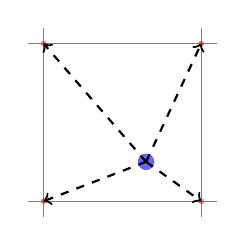
\begin{tikzpicture}[scale=1.0,transform shape,node distance=1cm]	
			\draw[very thin,color=gray,step=2cm] (-0.2,-0.2) grid (2.2,2.2);
			\fill[color=blue,opacity=0.6] (1.3,0.5) circle (3pt);
			\fill[color=red,opacity=0.6] (2.0,2.0) circle (1pt);
			\fill[color=red,opacity=0.6] (2.0,0.0) circle (1pt);
			\fill[color=red,opacity=0.6] (0.0,0.0) circle (1pt);
			\fill[color=red,opacity=0.6] (0.0,2.0) circle (1pt);
			
            \path[style=thick,dashed, ->] (1.3,0.5) edge (2.0,2.0);
            \path[style=thick,dashed, ->] (1.3,0.5) edge (2.0,0.0);
            \path[style=thick,dashed, ->] (1.3,0.5) edge (0.0,2.0);
            \path[style=thick,dashed, ->] (1.3,0.5) edge (0.0,0.0);

		\end{tikzpicture}

        \end{minipage} 
		\end{block}

		\vspace{0.5cm}
	
        \begin{itemize}
		\item Finite difference scheme leading to a set of linear equations
		\[
			\mathbf{A} \mathbf{x} = \mathbf{b} \text{,}
		\]
		$\textbf{b}$ denotes the charge densities on the mesh

        \item Integrated into code tracking relativistic particles in \alert{time}
        \end{itemize}

	\end{frame}
    
	\begin{frame}
		\frametitle{Goal}

		\begin{alertblock}{An efficient iterative solver for the Poisson equation on irrgular domains}
		\begin{itemize}
			\item Solve anisotropic electrostatic Poisson equation with an iterative solver
            \item Easy to specify boundary surface
			\item \alert{\textbf{Irregular}} domain imbedded in a rectangular domain
            \item ``Exact'' (Dirichlet) boundary conditions %(opposed to open boundary conditions FFT)
            \item Achieving good parallel efficiency
            \item Reuse information available from previous time steps
            \item Ref: Adelmann/Arbenz/Ineichen, J. Comp. Phys., 229, 4554-4566, 2010
            \item Similar to P. McCorquodale, P. Colella, D. P. Grote, J.-L. Vay, J. Comp. Phys., 201, 34-60, 2004
		\end{itemize}
		\end{alertblock}

	\end{frame}
	
    \section{Solver}

    \begin{frame}
        \frametitle{Solver in a Nutshell}

		\begin{columns}
		\begin{column}{5.5cm}
			\begin{itemize}
                \item Second order finite difference discretization leads to a large sparse linear system
                    \[
                            \mathbf{Ax} = \mathbf{b}
                    \]
                    with $\mathbf{A}$ (non-)symmteric positive definite.
				%\item standard 7 point stencil (3D) on Cartesian grid
				\item {\color{blue!60}Conjugent gradient} iterative solver
				\item Preconditioned by a smoothed aggregation-based {\color{blue!60}algebraic multigrid}
			\end{itemize}
		\end{column}
		\begin{column}{4.5cm}
            \centering
            % Sketch output, version 0.2 (build 27d, Sat Jan 26 23:58:07 2008)
% Output language: PGF/TikZ
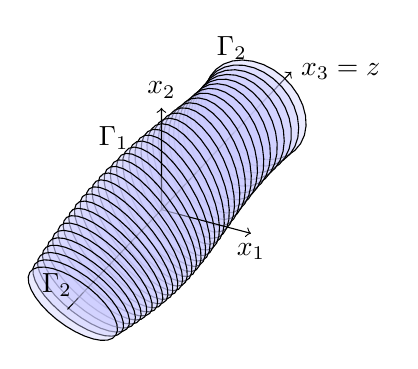
\begin{tikzpicture}[join=round,scale=0.6]
\draw[arrows=->,line width=.4pt](0,0)--(.758,.805);
\filldraw[fill=blue!20,fill opacity=0.4](.584,.697)--(.384,.847)--(.168,.959)--(-.056,1.029)--(-.277,1.055)--(-.487,1.034)--(-.675,.969)--(-.833,.86)--(-.955,.715)--(-1.036,.538)--(-1.071,.337)--(-1.059,.122)--(-1.001,-.099)--(-.899,-.315)--(-.758,-.517)--(-.584,-.697)--(-.384,-.847)--(-.168,-.959)--(.056,-1.029)--(.277,-1.055)--(.487,-1.034)--(.675,-.969)--(.833,-.86)--(.955,-.715)--(1.036,-.538)--(1.071,-.337)--(1.059,-.122)--(1.001,.099)--(.899,.315)--(.758,.517)--cycle;
\draw[arrows=-,line width=.4pt](-.114,-.121)--(0,0);
\filldraw[fill=blue!20,fill opacity=0.4](.38,.658)--(.181,.794)--(-.03,.89)--(-.245,.942)--(-.455,.948)--(-.649,.906)--(-.82,.82)--(-.96,.693)--(-1.064,.531)--(-1.125,.339)--(-1.143,.128)--(-1.115,-.094)--(-1.044,-.317)--(-.932,-.532)--(-.784,-.729)--(-.607,-.899)--(-.409,-1.035)--(-.197,-1.131)--(.018,-1.183)--(.227,-1.189)--(.422,-1.148)--(.593,-1.062)--(.733,-.935)--(.836,-.772)--(.898,-.581)--(.915,-.369)--(.888,-.147)--(.816,.076)--(.705,.291)--(.557,.488)--cycle;
\draw[arrows=-,line width=.4pt](-.227,-.241)--(-.114,-.121);
\filldraw[fill=blue!20,fill opacity=0.4](.175,.613)--(-.021,.735)--(-.227,.815)--(-.432,.849)--(-.629,.835)--(-.808,.774)--(-.961,.668)--(-1.083,.523)--(-1.167,.344)--(-1.21,.14)--(-1.211,-.081)--(-1.168,-.308)--(-1.084,-.533)--(-.962,-.746)--(-.809,-.936)--(-.63,-1.096)--(-.434,-1.218)--(-.228,-1.298)--(-.023,-1.331)--(.174,-1.317)--(.353,-1.256)--(.507,-1.151)--(.628,-1.006)--(.712,-.827)--(.756,-.623)--(.756,-.402)--(.713,-.174)--(.629,.051)--(.508,.263)--(.354,.453)--cycle;
\draw[arrows=-,line width=.4pt](-.341,-.362)--(-.227,-.241);
\filldraw[fill=blue!20,fill opacity=0.4](-.029,.562)--(-.223,.671)--(-.421,.734)--(-.617,.749)--(-.8,.716)--(-.963,.636)--(-1.099,.512)--(-1.201,.35)--(-1.267,.157)--(-1.291,-.059)--(-1.275,-.288)--(-1.217,-.52)--(-1.121,-.746)--(-.991,-.955)--(-.833,-1.137)--(-.653,-1.286)--(-.459,-1.395)--(-.261,-1.458)--(-.066,-1.474)--(.117,-1.44)--(.28,-1.36)--(.416,-1.236)--(.519,-1.074)--(.584,-.881)--(.609,-.665)--(.592,-.436)--(.535,-.204)--(.439,.022)--(.309,.23)--(.15,.413)--cycle;
\draw[arrows=-,line width=.4pt](-.455,-.483)--(-.341,-.362);
\filldraw[fill=blue!20,fill opacity=0.4](-.234,.505)--(-.423,.6)--(-.614,.647)--(-.798,.644)--(-.967,.593)--(-1.114,.494)--(-1.232,.353)--(-1.315,.175)--(-1.362,-.032)--(-1.368,-.258)--(-1.335,-.494)--(-1.263,-.73)--(-1.156,-.955)--(-1.018,-1.159)--(-.856,-1.333)--(-.676,-1.471)--(-.486,-1.565)--(-.296,-1.612)--(-.112,-1.61)--(.057,-1.558)--(.204,-1.46)--(.322,-1.318)--(.406,-1.14)--(.452,-.934)--(.459,-.707)--(.425,-.471)--(.354,-.236)--(.246,-.011)--(.109,.193)--(-.054,.368)--cycle;
\draw[arrows=-,line width=.4pt](-.569,-.603)--(-.455,-.483);
\filldraw[fill=blue!20,fill opacity=0.4](-.437,.443)--(-.622,.523)--(-.805,.553)--(-.977,.533)--(-1.131,.464)--(-1.261,.348)--(-1.36,.19)--(-1.425,-.003)--(-1.453,-.221)--(-1.442,-.457)--(-1.392,-.698)--(-1.307,-.936)--(-1.189,-1.159)--(-1.045,-1.358)--(-.879,-1.524)--(-.7,-1.65)--(-.515,-1.729)--(-.333,-1.76)--(-.16,-1.74)--(-.006,-1.671)--(.124,-1.555)--(.223,-1.397)--(.288,-1.204)--(.316,-.986)--(.304,-.75)--(.255,-.508)--(.17,-.271)--(.052,-.048)--(-.092,.151)--(-.258,.317)--cycle;
\draw[arrows=-,line width=.4pt](-.682,-.724)--(-.569,-.603);
\filldraw[fill=blue!20,fill opacity=0.4](-.639,.373)--(-.819,.439)--(-.992,.454)--(-1.152,.417)--(-1.291,.33)--(-1.404,.197)--(-1.485,.024)--(-1.531,-.182)--(-1.54,-.411)--(-1.512,-.654)--(-1.447,-.901)--(-1.349,-1.139)--(-1.221,-1.359)--(-1.07,-1.552)--(-.903,-1.708)--(-.725,-1.822)--(-.546,-1.887)--(-.373,-1.902)--(-.213,-1.865)--(-.073,-1.778)--(.039,-1.645)--(.12,-1.472)--(.166,-1.267)--(.175,-1.037)--(.147,-.794)--(.082,-.548)--(-.016,-.309)--(-.143,-.089)--(-.294,.104)--(-.462,.26)--cycle;
\draw[arrows=-,line width=.4pt](-.796,-.845)--(-.682,-.724);
\filldraw[fill=blue!20,fill opacity=0.4](-.84,.298)--(-1.013,.349)--(-1.177,.348)--(-1.323,.294)--(-1.447,.191)--(-1.543,.043)--(-1.605,-.144)--(-1.633,-.362)--(-1.624,-.601)--(-1.578,-.851)--(-1.499,-1.1)--(-1.388,-1.338)--(-1.252,-1.555)--(-1.096,-1.74)--(-.927,-1.887)--(-.752,-1.988)--(-.579,-2.039)--(-.415,-2.037)--(-.269,-1.984)--(-.145,-1.881)--(-.049,-1.732)--(.013,-1.545)--(.041,-1.327)--(.032,-1.088)--(-.014,-.839)--(-.093,-.59)--(-.204,-.351)--(-.34,-.135)--(-.496,.051)--(-.665,.197)--cycle;
\draw[arrows=-,line width=.4pt](-.91,-.966)--(-.796,-.845);
\filldraw[fill=blue!20,fill opacity=0.4](-1.039,.216)--(-1.205,.252)--(-1.358,.236)--(-1.491,.166)--(-1.599,.048)--(-1.677,-.115)--(-1.722,-.315)--(-1.731,-.544)--(-1.704,-.791)--(-1.642,-1.046)--(-1.548,-1.297)--(-1.427,-1.533)--(-1.283,-1.745)--(-1.122,-1.923)--(-.952,-2.059)--(-.781,-2.147)--(-.615,-2.183)--(-.462,-2.167)--(-.328,-2.097)--(-.22,-1.979)--(-.142,-1.816)--(-.098,-1.616)--(-.089,-1.387)--(-.116,-1.14)--(-.177,-.886)--(-.271,-.634)--(-.393,-.398)--(-.537,-.186)--(-.697,-.008)--(-.867,.128)--cycle;
\draw[arrows=-,line width=.4pt](-1.023,-1.086)--(-.91,-.966);
\filldraw[fill=blue!20,fill opacity=0.4](-1.235,.127)--(-1.393,.149)--(-1.535,.118)--(-1.655,.033)--(-1.747,-.1)--(-1.808,-.277)--(-1.834,-.488)--(-1.825,-.726)--(-1.781,-.98)--(-1.703,-1.238)--(-1.596,-1.49)--(-1.464,-1.724)--(-1.313,-1.93)--(-1.149,-2.099)--(-.98,-2.224)--(-.812,-2.3)--(-.654,-2.322)--(-.512,-2.29)--(-.392,-2.206)--(-.3,-2.072)--(-.239,-1.896)--(-.213,-1.684)--(-.222,-1.446)--(-.266,-1.192)--(-.343,-.934)--(-.45,-.682)--(-.582,-.448)--(-.734,-.242)--(-.898,-.073)--(-1.067,.052)--cycle;
\draw[arrows=-,line width=.4pt](-1.137,-1.207)--(-1.023,-1.086);
\filldraw[fill=blue!20,fill opacity=0.4](-1.428,.032)--(-1.578,.04)--(-1.709,-.006)--(-1.815,-.105)--(-1.891,-.252)--(-1.934,-.441)--(-1.943,-.663)--(-1.916,-.909)--(-1.855,-1.168)--(-1.763,-1.429)--(-1.643,-1.68)--(-1.501,-1.91)--(-1.344,-2.11)--(-1.177,-2.27)--(-1.009,-2.384)--(-.846,-2.446)--(-.696,-2.454)--(-.565,-2.407)--(-.459,-2.308)--(-.383,-2.161)--(-.34,-1.973)--(-.332,-1.75)--(-.359,-1.504)--(-.419,-1.245)--(-.512,-.985)--(-.631,-.734)--(-.773,-.504)--(-.931,-.304)--(-1.097,-.144)--(-1.266,-.03)--cycle;
\draw[arrows=-,line width=.4pt](-1.251,-1.328)--(-1.137,-1.207);
\filldraw[fill=blue!20,fill opacity=0.4](-1.619,-.07)--(-1.76,-.076)--(-1.879,-.136)--(-1.97,-.249)--(-2.03,-.409)--(-2.056,-.608)--(-2.047,-.84)--(-2.003,-1.092)--(-1.926,-1.355)--(-1.82,-1.617)--(-1.689,-1.866)--(-1.538,-2.092)--(-1.375,-2.284)--(-1.207,-2.434)--(-1.04,-2.536)--(-.883,-2.585)--(-.742,-2.579)--(-.623,-2.519)--(-.531,-2.406)--(-.471,-2.247)--(-.445,-2.047)--(-.455,-1.815)--(-.499,-1.563)--(-.576,-1.3)--(-.682,-1.038)--(-.813,-.789)--(-.964,-.563)--(-1.127,-.371)--(-1.295,-.221)--(-1.461,-.119)--cycle;
\draw[arrows=-,line width=.4pt](-1.365,-1.448)--(-1.251,-1.328);
\filldraw[fill=blue!20,fill opacity=0.4](-1.806,-.178)--(-1.937,-.198)--(-2.044,-.272)--(-2.121,-.397)--(-2.165,-.568)--(-2.174,-.778)--(-2.148,-1.017)--(-2.087,-1.275)--(-1.995,-1.541)--(-1.875,-1.802)--(-1.733,-2.048)--(-1.575,-2.268)--(-1.408,-2.452)--(-1.238,-2.592)--(-1.075,-2.682)--(-.924,-2.718)--(-.792,-2.699)--(-.685,-2.625)--(-.608,-2.499)--(-.564,-2.328)--(-.555,-2.118)--(-.581,-1.879)--(-.642,-1.621)--(-.734,-1.356)--(-.854,-1.094)--(-.996,-.848)--(-1.154,-.628)--(-1.321,-.444)--(-1.491,-.304)--(-1.655,-.214)--cycle;
\draw[arrows=-,line width=.4pt](-1.478,-1.569)--(-1.365,-1.448);
\filldraw[fill=blue!20,fill opacity=0.4](-1.989,-.293)--(-2.111,-.326)--(-2.205,-.412)--(-2.268,-.55)--(-2.296,-.732)--(-2.288,-.95)--(-2.245,-1.196)--(-2.169,-1.458)--(-2.062,-1.725)--(-1.93,-1.985)--(-1.778,-2.226)--(-1.613,-2.439)--(-1.442,-2.614)--(-1.272,-2.744)--(-1.112,-2.822)--(-.968,-2.845)--(-.846,-2.812)--(-.751,-2.725)--(-.689,-2.588)--(-.661,-2.406)--(-.668,-2.187)--(-.711,-1.942)--(-.788,-1.68)--(-.895,-1.413)--(-1.027,-1.153)--(-1.179,-.912)--(-1.344,-.699)--(-1.515,-.524)--(-1.684,-.394)--(-1.845,-.316)--cycle;
\draw[arrows=-,line width=.4pt](-1.592,-1.69)--(-1.478,-1.569);
\filldraw[fill=blue!20,fill opacity=0.4](-2.168,-.414)--(-2.28,-.46)--(-2.362,-.559)--(-2.41,-.707)--(-2.422,-.899)--(-2.398,-1.125)--(-2.339,-1.375)--(-2.247,-1.64)--(-2.127,-1.906)--(-1.983,-2.163)--(-1.822,-2.4)--(-1.651,-2.605)--(-1.478,-2.771)--(-1.309,-2.889)--(-1.153,-2.955)--(-1.016,-2.965)--(-.904,-2.92)--(-.822,-2.821)--(-.774,-2.672)--(-.762,-2.481)--(-.786,-2.255)--(-.845,-2.004)--(-.937,-1.74)--(-1.057,-1.473)--(-1.201,-1.216)--(-1.362,-.979)--(-1.533,-.774)--(-1.707,-.609)--(-1.875,-.49)--(-2.031,-.425)--cycle;
\draw[arrows=-,line width=.4pt](-1.706,-1.81)--(-1.592,-1.69);
\filldraw[fill=blue!20,fill opacity=0.4](-2.344,-.542)--(-2.445,-.599)--(-2.514,-.71)--(-2.547,-.868)--(-2.544,-1.068)--(-2.505,-1.3)--(-2.43,-1.555)--(-2.324,-1.82)--(-2.19,-2.086)--(-2.036,-2.339)--(-1.867,-2.569)--(-1.691,-2.766)--(-1.516,-2.921)--(-1.348,-3.028)--(-1.197,-3.081)--(-1.068,-3.079)--(-.967,-3.022)--(-.898,-2.911)--(-.864,-2.752)--(-.867,-2.553)--(-.907,-2.32)--(-.982,-2.066)--(-1.088,-1.8)--(-1.221,-1.535)--(-1.376,-1.282)--(-1.545,-1.052)--(-1.721,-.855)--(-1.896,-.7)--(-2.063,-.593)--(-2.214,-.54)--cycle;
\draw[arrows=-,line width=.4pt](-1.819,-1.931)--(-1.706,-1.81);
\filldraw[fill=blue!20,fill opacity=0.4](-2.514,-.675)--(-2.605,-.744)--(-2.661,-.866)--(-2.68,-1.033)--(-2.662,-1.24)--(-2.607,-1.477)--(-2.518,-1.734)--(-2.398,-2)--(-2.252,-2.262)--(-2.088,-2.51)--(-1.912,-2.733)--(-1.732,-2.921)--(-1.556,-3.065)--(-1.391,-3.16)--(-1.245,-3.201)--(-1.125,-3.187)--(-1.034,-3.118)--(-.978,-2.997)--(-.959,-2.829)--(-.977,-2.622)--(-1.032,-2.385)--(-1.121,-2.128)--(-1.241,-1.862)--(-1.387,-1.6)--(-1.551,-1.352)--(-1.727,-1.129)--(-1.907,-.941)--(-2.083,-.797)--(-2.248,-.702)--(-2.393,-.661)--cycle;
\draw[arrows=-,line width=.4pt](-1.933,-2.052)--(-1.819,-1.931);
\filldraw[fill=blue!20,fill opacity=0.4](-2.681,-.814)--(-2.76,-.895)--(-2.803,-1.026)--(-2.809,-1.202)--(-2.776,-1.415)--(-2.706,-1.655)--(-2.602,-1.914)--(-2.469,-2.178)--(-2.313,-2.436)--(-2.14,-2.678)--(-1.958,-2.893)--(-1.775,-3.07)--(-1.599,-3.204)--(-1.438,-3.286)--(-1.298,-3.315)--(-1.186,-3.289)--(-1.106,-3.209)--(-1.063,-3.078)--(-1.058,-2.902)--(-1.091,-2.689)--(-1.16,-2.448)--(-1.264,-2.19)--(-1.397,-1.926)--(-1.553,-1.667)--(-1.726,-1.425)--(-1.908,-1.211)--(-2.091,-1.033)--(-2.267,-.9)--(-2.428,-.817)--(-2.568,-.788)--cycle;
\draw[arrows=-,line width=.4pt](-2.047,-2.172)--(-1.933,-2.052);
\draw[arrows=<->,line width=.4pt](-.095,-2.615)--(-1.99,-2.112)--(-1.99,.043);
\filldraw[fill=blue!20,fill opacity=0.4](-2.842,-.959)--(-2.91,-1.05)--(-2.941,-1.19)--(-2.932,-1.373)--(-2.885,-1.591)--(-2.801,-1.834)--(-2.684,-2.092)--(-2.54,-2.354)--(-2.373,-2.607)--(-2.193,-2.842)--(-2.006,-3.047)--(-1.821,-3.214)--(-1.646,-3.336)--(-1.488,-3.407)--(-1.355,-3.423)--(-1.252,-3.385)--(-1.183,-3.294)--(-1.153,-3.155)--(-1.161,-2.972)--(-1.209,-2.754)--(-1.293,-2.511)--(-1.409,-2.253)--(-1.554,-1.991)--(-1.72,-1.737)--(-1.901,-1.503)--(-2.088,-1.298)--(-2.273,-1.13)--(-2.448,-1.009)--(-2.606,-.938)--(-2.739,-.921)--cycle;
\draw[arrows=-,line width=.4pt](-2.161,-2.293)--(-2.047,-2.172);
\filldraw[fill=blue!20,fill opacity=0.4](-2.999,-1.11)--(-3.056,-1.211)--(-3.073,-1.359)--(-3.051,-1.548)--(-2.99,-1.769)--(-2.893,-2.014)--(-2.764,-2.27)--(-2.608,-2.528)--(-2.433,-2.775)--(-2.246,-3.002)--(-2.055,-3.197)--(-1.869,-3.353)--(-1.696,-3.462)--(-1.542,-3.521)--(-1.416,-3.525)--(-1.323,-3.476)--(-1.266,-3.376)--(-1.248,-3.228)--(-1.27,-3.039)--(-1.331,-2.817)--(-1.428,-2.573)--(-1.557,-2.316)--(-1.713,-2.058)--(-1.888,-1.811)--(-2.075,-1.585)--(-2.266,-1.389)--(-2.452,-1.233)--(-2.626,-1.124)--(-2.779,-1.066)--(-2.905,-1.061)--cycle;
\draw[arrows=-,line width=.4pt](-2.274,-2.414)--(-2.161,-2.293);
\filldraw[fill=blue!20,fill opacity=0.4](-3.15,-1.265)--(-3.196,-1.375)--(-3.201,-1.531)--(-3.166,-1.725)--(-3.092,-1.949)--(-2.982,-2.193)--(-2.841,-2.447)--(-2.676,-2.7)--(-2.493,-2.94)--(-2.3,-3.157)--(-2.106,-3.341)--(-1.92,-3.486)--(-1.749,-3.583)--(-1.601,-3.629)--(-1.482,-3.622)--(-1.398,-3.562)--(-1.353,-3.452)--(-1.347,-3.297)--(-1.382,-3.103)--(-1.457,-2.879)--(-1.566,-2.635)--(-1.707,-2.381)--(-1.873,-2.128)--(-2.056,-1.888)--(-2.249,-1.671)--(-2.442,-1.486)--(-2.629,-1.342)--(-2.8,-1.245)--(-2.948,-1.199)--(-3.066,-1.206)--cycle;
\draw[arrows=-,line width=.4pt](-2.388,-2.534)--(-2.274,-2.414);
\filldraw[fill=blue!20,fill opacity=0.4](-3.297,-1.426)--(-3.331,-1.544)--(-3.324,-1.706)--(-3.276,-1.904)--(-3.19,-2.129)--(-3.068,-2.372)--(-2.917,-2.623)--(-2.742,-2.869)--(-2.552,-3.101)--(-2.355,-3.308)--(-2.159,-3.481)--(-1.974,-3.613)--(-1.806,-3.698)--(-1.664,-3.731)--(-1.553,-3.713)--(-1.479,-3.643)--(-1.445,-3.525)--(-1.452,-3.363)--(-1.5,-3.165)--(-1.586,-2.94)--(-1.708,-2.697)--(-1.859,-2.446)--(-2.034,-2.2)--(-2.224,-1.968)--(-2.421,-1.761)--(-2.617,-1.588)--(-2.802,-1.456)--(-2.97,-1.371)--(-3.112,-1.337)--(-3.223,-1.356)--cycle;
\draw[arrows=-,line width=.4pt](-2.502,-2.655)--(-2.388,-2.534);
\filldraw[fill=blue!20,fill opacity=0.4](-3.438,-1.591)--(-3.461,-1.717)--(-3.442,-1.884)--(-3.382,-2.085)--(-3.284,-2.31)--(-3.151,-2.551)--(-2.99,-2.796)--(-2.808,-3.036)--(-2.612,-3.258)--(-2.412,-3.454)--(-2.215,-3.615)--(-2.031,-3.735)--(-1.867,-3.807)--(-1.732,-3.829)--(-1.629,-3.799)--(-1.565,-3.719)--(-1.542,-3.593)--(-1.561,-3.426)--(-1.621,-3.226)--(-1.719,-3)--(-1.852,-2.759)--(-2.013,-2.514)--(-2.195,-2.275)--(-2.391,-2.052)--(-2.592,-1.856)--(-2.788,-1.695)--(-2.973,-1.576)--(-3.136,-1.504)--(-3.272,-1.482)--(-3.374,-1.511)--cycle;
\draw[arrows=-,line width=.4pt](-2.615,-2.776)--(-2.502,-2.655);
\filldraw[fill=blue!20,fill opacity=0.4](-3.574,-1.76)--(-3.586,-1.893)--(-3.556,-2.065)--(-3.484,-2.267)--(-3.375,-2.492)--(-3.232,-2.729)--(-3.062,-2.969)--(-2.873,-3.199)--(-2.673,-3.412)--(-2.47,-3.596)--(-2.273,-3.745)--(-2.091,-3.851)--(-1.933,-3.911)--(-1.804,-3.92)--(-1.71,-3.88)--(-1.656,-3.792)--(-1.645,-3.659)--(-1.675,-3.487)--(-1.747,-3.284)--(-1.856,-3.06)--(-1.999,-2.822)--(-2.168,-2.583)--(-2.358,-2.352)--(-2.558,-2.14)--(-2.761,-1.955)--(-2.958,-1.807)--(-3.139,-1.7)--(-3.298,-1.641)--(-3.427,-1.631)--(-3.521,-1.672)--cycle;
\draw[arrows=-,line width=.4pt](-2.729,-2.897)--(-2.615,-2.776);
\filldraw[fill=blue!20,fill opacity=0.4](-3.705,-1.933)--(-3.707,-2.073)--(-3.665,-2.248)--(-3.582,-2.451)--(-3.462,-2.674)--(-3.31,-2.907)--(-3.133,-3.139)--(-2.938,-3.36)--(-2.734,-3.562)--(-2.53,-3.734)--(-2.334,-3.87)--(-2.156,-3.963)--(-2.002,-4.009)--(-1.881,-4.007)--(-1.796,-3.957)--(-1.753,-3.86)--(-1.752,-3.721)--(-1.793,-3.546)--(-1.876,-3.342)--(-1.996,-3.119)--(-2.148,-2.887)--(-2.325,-2.654)--(-2.52,-2.433)--(-2.724,-2.231)--(-2.929,-2.059)--(-3.124,-1.923)--(-3.303,-1.83)--(-3.456,-1.784)--(-3.577,-1.786)--(-3.662,-1.836)--cycle;
\draw[arrows=-,line width=.4pt](-2.843,-3.017)--(-2.729,-2.897);
\filldraw[fill=blue!20,fill opacity=0.4](-3.831,-2.11)--(-3.822,-2.255)--(-3.769,-2.432)--(-3.676,-2.636)--(-3.547,-2.856)--(-3.387,-3.083)--(-3.203,-3.307)--(-3.003,-3.518)--(-2.796,-3.708)--(-2.592,-3.867)--(-2.398,-3.989)--(-2.224,-4.069)--(-2.077,-4.103)--(-1.963,-4.089)--(-1.888,-4.029)--(-1.854,-3.924)--(-1.864,-3.78)--(-1.916,-3.602)--(-2.009,-3.399)--(-2.139,-3.179)--(-2.299,-2.952)--(-2.483,-2.728)--(-2.683,-2.516)--(-2.889,-2.327)--(-3.094,-2.167)--(-3.288,-2.045)--(-3.462,-1.965)--(-3.609,-1.931)--(-3.723,-1.945)--(-3.798,-2.006)--cycle;
\draw[arrows=-,line width=.4pt](-2.957,-3.138)--(-2.843,-3.017);
\filldraw[fill=blue!20,fill opacity=0.4](-3.952,-2.29)--(-3.932,-2.439)--(-3.869,-2.619)--(-3.767,-2.821)--(-3.629,-3.037)--(-3.461,-3.257)--(-3.272,-3.472)--(-3.068,-3.673)--(-2.86,-3.85)--(-2.656,-3.996)--(-2.465,-4.104)--(-2.296,-4.171)--(-2.155,-4.192)--(-2.05,-4.167)--(-1.984,-4.097)--(-1.961,-3.985)--(-1.981,-3.837)--(-2.044,-3.657)--(-2.146,-3.455)--(-2.285,-3.239)--(-2.452,-3.019)--(-2.642,-2.804)--(-2.845,-2.603)--(-3.053,-2.426)--(-3.257,-2.28)--(-3.448,-2.171)--(-3.617,-2.105)--(-3.758,-2.084)--(-3.863,-2.109)--(-3.929,-2.179)--cycle;
\draw[arrows=-,line width=.4pt](-3.07,-3.259)--(-2.957,-3.138);
\filldraw[fill=blue!20,fill opacity=0.4](-4.068,-2.474)--(-4.038,-2.626)--(-3.965,-2.806)--(-3.854,-3.006)--(-3.708,-3.217)--(-3.534,-3.43)--(-3.34,-3.635)--(-3.134,-3.824)--(-2.925,-3.988)--(-2.723,-4.12)--(-2.536,-4.215)--(-2.372,-4.268)--(-2.239,-4.276)--(-2.142,-4.241)--(-2.086,-4.162)--(-2.072,-4.044)--(-2.103,-3.891)--(-2.175,-3.711)--(-2.287,-3.511)--(-2.433,-3.3)--(-2.607,-3.087)--(-2.801,-2.882)--(-3.007,-2.693)--(-3.215,-2.529)--(-3.418,-2.397)--(-3.605,-2.302)--(-3.768,-2.25)--(-3.902,-2.241)--(-3.999,-2.277)--(-4.055,-2.355)--cycle;
\draw[arrows=-,line width=.4pt](-3.184,-3.379)--(-3.07,-3.259);
\filldraw[fill=blue!20,fill opacity=0.4](-4.179,-2.659)--(-4.139,-2.814)--(-4.057,-2.994)--(-3.937,-3.191)--(-3.784,-3.396)--(-3.605,-3.601)--(-3.408,-3.795)--(-3.2,-3.972)--(-2.992,-4.122)--(-2.793,-4.24)--(-2.61,-4.321)--(-2.452,-4.36)--(-2.327,-4.357)--(-2.239,-4.31)--(-2.192,-4.223)--(-2.189,-4.1)--(-2.229,-3.944)--(-2.311,-3.764)--(-2.431,-3.567)--(-2.584,-3.362)--(-2.763,-3.158)--(-2.96,-2.963)--(-3.168,-2.787)--(-3.376,-2.636)--(-3.576,-2.518)--(-3.758,-2.438)--(-3.916,-2.398)--(-4.041,-2.402)--(-4.129,-2.448)--(-4.176,-2.535)--cycle;
\draw[arrows=-,line width=.4pt](-3.298,-3.5)--(-3.184,-3.379);
\filldraw[fill=blue!20,fill opacity=0.4](-4.285,-2.847)--(-4.236,-3.004)--(-4.145,-3.183)--(-4.018,-3.376)--(-3.859,-3.574)--(-3.675,-3.769)--(-3.475,-3.953)--(-3.267,-4.116)--(-3.061,-4.253)--(-2.865,-4.356)--(-2.688,-4.423)--(-2.537,-4.449)--(-2.42,-4.433)--(-2.341,-4.377)--(-2.304,-4.282)--(-2.31,-4.153)--(-2.36,-3.996)--(-2.45,-3.817)--(-2.578,-3.624)--(-2.737,-3.426)--(-2.92,-3.231)--(-3.12,-3.047)--(-3.328,-2.884)--(-3.534,-2.747)--(-3.731,-2.644)--(-3.908,-2.577)--(-4.058,-2.551)--(-4.176,-2.567)--(-4.255,-2.623)--(-4.292,-2.718)--cycle;
\draw[arrows=-,line width=.4pt](-3.411,-3.621)--(-3.298,-3.5);
\filldraw[fill=blue!20,fill opacity=0.4](-4.387,-3.036)--(-4.328,-3.195)--(-4.23,-3.372)--(-4.096,-3.56)--(-3.931,-3.751)--(-3.745,-3.936)--(-3.543,-4.107)--(-3.336,-4.257)--(-3.132,-4.379)--(-2.94,-4.468)--(-2.769,-4.52)--(-2.626,-4.533)--(-2.517,-4.506)--(-2.448,-4.44)--(-2.42,-4.338)--(-2.436,-4.205)--(-2.494,-4.046)--(-2.593,-3.869)--(-2.727,-3.681)--(-2.891,-3.49)--(-3.078,-3.305)--(-3.28,-3.134)--(-3.487,-2.984)--(-3.691,-2.862)--(-3.883,-2.773)--(-4.054,-2.721)--(-4.197,-2.709)--(-4.306,-2.736)--(-4.375,-2.802)--(-4.403,-2.903)--cycle;
\draw[arrows=-,line width=.4pt](-3.525,-3.741)--(-3.411,-3.621);
\filldraw[fill=blue!20,fill opacity=0.4](-4.484,-3.227)--(-4.417,-3.386)--(-4.311,-3.561)--(-4.171,-3.743)--(-4.002,-3.926)--(-3.813,-4.1)--(-3.611,-4.258)--(-3.405,-4.394)--(-3.205,-4.502)--(-3.019,-4.576)--(-2.854,-4.614)--(-2.719,-4.614)--(-2.62,-4.575)--(-2.559,-4.5)--(-2.541,-4.392)--(-2.566,-4.255)--(-2.633,-4.096)--(-2.739,-3.922)--(-2.88,-3.739)--(-3.048,-3.557)--(-3.237,-3.383)--(-3.439,-3.224)--(-3.645,-3.088)--(-3.845,-2.981)--(-4.032,-2.907)--(-4.196,-2.869)--(-4.331,-2.869)--(-4.431,-2.908)--(-4.491,-2.983)--(-4.509,-3.091)--cycle;
\draw[arrows=-,line width=.4pt](-3.639,-3.862)--(-3.525,-3.741);
\filldraw[fill=blue!20,fill opacity=0.4](-4.576,-3.419)--(-4.502,-3.578)--(-4.389,-3.749)--(-4.244,-3.925)--(-4.072,-4.098)--(-3.881,-4.261)--(-3.68,-4.407)--(-3.477,-4.528)--(-3.281,-4.621)--(-3.1,-4.68)--(-2.943,-4.704)--(-2.817,-4.691)--(-2.727,-4.641)--(-2.676,-4.558)--(-2.667,-4.444)--(-2.701,-4.305)--(-2.776,-4.146)--(-2.889,-3.975)--(-3.034,-3.799)--(-3.206,-3.626)--(-3.397,-3.463)--(-3.598,-3.317)--(-3.801,-3.196)--(-3.997,-3.103)--(-4.177,-3.044)--(-4.334,-3.02)--(-4.461,-3.033)--(-4.551,-3.083)--(-4.602,-3.166)--(-4.61,-3.28)--cycle;
\draw[arrows=-,line width=.4pt](-3.753,-3.983)--(-3.639,-3.862);
\filldraw[fill=blue!20,fill opacity=0.4](-4.665,-3.612)--(-4.583,-3.77)--(-4.464,-3.936)--(-4.314,-4.105)--(-4.14,-4.269)--(-3.949,-4.42)--(-3.749,-4.552)--(-3.549,-4.659)--(-3.359,-4.736)--(-3.185,-4.781)--(-3.036,-4.79)--(-2.919,-4.765)--(-2.838,-4.705)--(-2.797,-4.614)--(-2.798,-4.495)--(-2.84,-4.353)--(-2.923,-4.196)--(-3.041,-4.029)--(-3.191,-3.86)--(-3.365,-3.697)--(-3.556,-3.546)--(-3.756,-3.414)--(-3.956,-3.307)--(-4.146,-3.229)--(-4.32,-3.185)--(-4.469,-3.175)--(-4.586,-3.201)--(-4.667,-3.261)--(-4.708,-3.352)--(-4.707,-3.471)--cycle;
\draw[arrows=-,line width=.4pt](-3.866,-4.103)--(-3.753,-3.983);
\filldraw[fill=blue!20,fill opacity=0.4](-4.75,-3.805)--(-4.66,-3.961)--(-4.536,-4.123)--(-4.383,-4.284)--(-4.207,-4.437)--(-4.017,-4.575)--(-3.819,-4.693)--(-3.624,-4.785)--(-3.44,-4.848)--(-3.274,-4.878)--(-3.133,-4.874)--(-3.025,-4.836)--(-2.954,-4.766)--(-2.923,-4.668)--(-2.932,-4.544)--(-2.983,-4.402)--(-3.072,-4.246)--(-3.196,-4.084)--(-3.349,-3.923)--(-3.525,-3.77)--(-3.716,-3.632)--(-3.913,-3.514)--(-4.108,-3.421)--(-4.293,-3.359)--(-4.459,-3.329)--(-4.599,-3.333)--(-4.707,-3.371)--(-4.779,-3.441)--(-4.81,-3.539)--(-4.8,-3.663)--cycle;
\draw[arrows=-,line width=.4pt](-3.98,-4.224)--(-3.866,-4.103);
\path (.758,.805) node[right] {$x_3 = z$}
                   (-.095,-2.615) node[below] {$x_1$}
                   (-1.99,.043) node[above] {$x_2$};


\node at (-4.2,-3.7) {$\Gamma_2$};
\node at (-3.0,-0.6) {$\Gamma_1$};
\node at (-0.5, 1.3) {$\Gamma_2$};
\end{tikzpicture}% End sketch output

		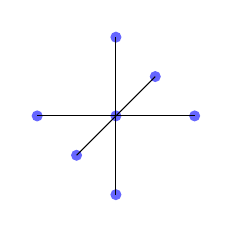
\begin{tikzpicture}[scale=0.5, join=round, transform shape,node distance=1cm]	
            \coordinate (C) at (0,0);
            \coordinate (E) at (2,0);
            \coordinate (W) at (-2,0);
            \coordinate (N) at (0,2);
            \coordinate (S) at (0,-2);
            \coordinate (F) at (-1,-1);
            \coordinate (B) at (1,1);
            
            \fill[blue!60] (C) circle (4pt);
            \draw (C) node[above left] {};
            \fill[blue!60] (E) circle (4pt);
            \draw (C) -- (E) node[right] {};
            \fill[blue!60] (W) circle (4pt);
            \draw (C) -- (W) node[left] {};
            \fill[blue!60] (N) circle (4pt);
            \draw (C) -- (N) node[above] {};
            \fill[blue!60] (S) circle (4pt);
            \draw (C) -- (S) node[below] {};
            \fill[blue!60] (F) circle (4pt);
            \draw (C) -- (F) node[below left] {};
            \fill[blue!60] (B) circle (4pt);
            \draw (C) -- (B) node[above right] {};
		
        \end{tikzpicture}
		\end{column}
		\end{columns}

    \end{frame}

	
	\begin{frame}
		\frametitle{AMG Parameters}
			
        \begin{minipage}[b]{0.6\textwidth}
			\begin{itemize}
			    \item ``Decoupled'' {\color{blue!60}aggregation scheme}: aggregates of size $3\times3\times3$
                \begin{itemize}
    				\item Each processor aggregate its portion of the grid
	    			\item Many aggregates near inter-processor boundaries with non-optimal size
			    	\item Number of vertices is substantially reduced in every coarsening step
		    		%\item number of processors determine number of aggregates: coarse problem may still be to big
				    %IFF: memory consumption for SA AMG prec AND linear system matrix A_0 \approx 1.5*Storage(A_0)
    				%\item typical operator complexity for decoupled aggregation is $1.5$
                \end{itemize}
            \end{itemize}
        \end{minipage}
        \begin{minipage}[b]{0.3\textwidth}
        \centering
                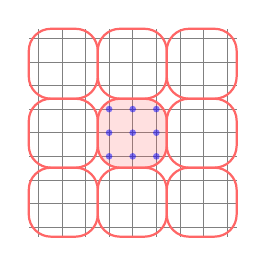
\begin{tikzpicture}[scale=0.6]
                    \draw[very thin,color=gray,step=5mm] (-0.2,-0.2) grid (4.2,4.2);

                    \draw[thick,rounded corners=8pt,color=red!60,fill=red!60,opacity=0.2] (1.26,1.26) rectangle (2.72,2.72);
                    \draw[thick,rounded corners=8pt,color=red!60] (1.26,1.26) rectangle (2.72,2.72);
                    \draw[thick,rounded corners=8pt,color=red!60] (4.2,4.2) rectangle (2.72,2.72);
                    \draw[thick,rounded corners=8pt,color=red!60] (4.2,1.26) rectangle (2.72,2.72);
                    \draw[thick,rounded corners=8pt,color=red!60] (1.26,4.2) rectangle (2.72,2.72);
                    \draw[thick,rounded corners=8pt,color=red!60] (-0.2,4.2) rectangle (1.26,2.72);
                    \draw[thick,rounded corners=8pt,color=red!60] (-0.2,2.72) rectangle (1.26,1.26);
                    \draw[thick,rounded corners=8pt,color=red!60] (-0.2,-0.2) rectangle (1.26,1.26);
                    \draw[thick,rounded corners=8pt,color=red!60] (1.26,-0.2) rectangle (2.72,1.26);
                    \draw[thick,rounded corners=8pt,color=red!60] (2.72,-0.2) rectangle (4.2,1.26);
			
                    \fill[color=blue,opacity=0.5] (1.5,1.5) circle (2pt);
                    \fill[color=blue,opacity=0.5] (1.5,2.0) circle (2pt);
                    \fill[color=blue,opacity=0.5] (1.5,2.5) circle (2pt);
                    \fill[color=blue,opacity=0.5] (2.0,1.5) circle (2pt);
                    \fill[color=blue,opacity=0.5] (2.0,2.0) circle (2pt);
                    \fill[color=blue,opacity=0.5] (2.0,2.5) circle (2pt);
                    \fill[color=blue,opacity=0.5] (2.5,1.5) circle (2pt);
                    \fill[color=blue,opacity=0.5] (2.5,2.0) circle (2pt);
                    \fill[color=blue,opacity=0.5] (2.5,2.5) circle (2pt);

                \end{tikzpicture}
                \scriptsize{\\clustering vertices into aggregates}

        \end{minipage} 
        \begin{itemize}
			    \item Chebyshev polynomial {\color{blue!60}pre and postsmoothers} perform well for parallel solvers (M. Adams, M. Brezina, J. Hu, R. Tuminaro, J. Comp. Phys., 2003)
    		    \item LU based direct {\color{blue!60}coarse level solver}
                \item V-cycle
        \end{itemize}

            \vspace{0.3cm}
            \alert{AMG performance critically depends on choice of parameters!}

	\end{frame}

	\begin{frame}
		\frametitle{Implementation (1/2)}

		For preconditioner setup and iterative solver we used \textsc{Trilinos}:
		\begin{itemize}
			\item \textsc{Epetra}: distributed matrices and vectors
			\item \textsc{Amesos}: direct coarse level solver
			\item \textsc{AztecOO}: iterative solver
			\item \textsc{ML}: smoothed aggregation based AMG preconditioner
		\end{itemize}

		\vspace{0.8cm}

		\opal in conjunction with Independent Parallel Particle Layer (\textsc{IP$^2$L}) offers:
		\begin{itemize}
			\item parallel fields
			\item particle representation
			\item operators on fields and particles
		\end{itemize}

	\end{frame}

	\begin{frame}
		\frametitle{Implementation (2/2)}
		\framesubtitle{Integrating the Solver in \opal}

		\begin{center}
		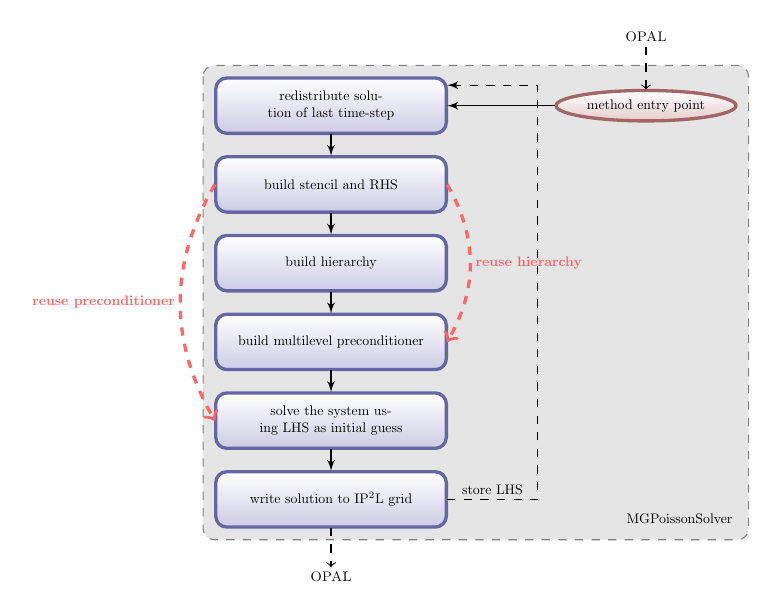
\begin{tikzpicture}[scale=0.5, transform shape, node distance = 2cm, auto]
			\tikzstyle{decision} = [diamond, draw, fill=blue!20, text width=12em, text badly centered, node distance=3cm, inner sep=0pt]
			\tikzstyle{block} = [rectangle, draw, fill=blue!20, text width=16em, text centered, rounded corners, minimum height=4em, shade,top color=white,bottom color=blue!50!black!20, draw=blue!40!black!60, very thick]
			\tikzstyle{line} = [draw, -latex'];
			\tikzstyle{cloud} = [draw, ellipse, node distance=8cm, minimum height=2em, shade, top color=white,bottom color=red!50!black!20, draw=red!40!black!60, very thick];
			
			\node [block] (redistSol) {redistribute solution of last time-step};
			\node [cloud, right of=redistSol] (entry) {method entry point};
			\node [block, below of=redistSol] (stencil) {build stencil and RHS};
            \node [block, below of=stencil] (hier) {build hierarchy};
			\node [block, below of=hier] (ml) {build multilevel preconditioner};
			\node [block, below of=ml] (solve) {solve the system using LHS as initial guess};
			\node [block, below of=solve] (lhs) {write solution to IP$^2$L grid};
			%\node [decision, below of=evaluate] (decide) {is best candidate better?};
			\path [line] (redistSol) -- (stencil);
			\path [line] (stencil) -- (hier);
			\path [line] (hier) -- (ml);
			\path [line] (ml) -- (solve);
			\path [line] (solve) -- (lhs);
			\path [line] (entry) -- (redistSol);
			\path [line,dashed] (lhs.east) -- node {store LHS} + (2.3,0.0) |- (redistSol.370);
			\path [->,dashed,color=red!60,very thick] (stencil.west) edge [bend right] node [left]{\textbf{reuse preconditioner}} (solve.west);
			\path [->,dashed,color=red!60,very thick] (stencil.east) edge [bend left] node {\textbf{reuse hierarchy}} (ml.east);

			\draw [<-,dashed] (entry) -- node [above, text width=5em] {} + (0,1.5) node[above] {\opal};
			\draw [->,dashed] (lhs.270) -- node [above, text width=5em] {} + (0,-1.0) node[below] {\opal};


			\begin{pgfonlayer}{background}
        			\path (redistSol.north west)+(-0.3,0.3) node (a) {};
			        \path (lhs.south -| entry.east)+(+0.3,-0.3) node (b) {};
			        \path[fill=black!10,rounded corners, draw=black!50, dashed] (a) rectangle (b);
			        \path (lhs.east)+(5.9,-0.5) node (name) {MGPoissonSolver};
			\end{pgfonlayer}

		\end{tikzpicture}
		\end{center}

	\end{frame}



    \section{Boundary Conditions}
	
	\begin{frame}
		\frametitle{Boundary Conditions}

		\begin{columns}
		\begin{column}{5cm}

		\begin{block}{Boundary Problem}
    		%\begin{eqnarray*}
            \[
	    		\nabla^2 \phi = -\frac{\rho}{\epsilon_0} \text{, in } \Omega \subset \Re^3 , \nonumber 
            \]
            \[
                \phi = 0 \text{, on }\Gamma_1  
            \]
            \[
                \frac{\partial \phi}{\partial \vec{n}} + \frac {1}{d} \phi = 0  \text{, on } \Gamma_2
            \]
    		%\end{eqnarray*}
		\end{block}
        \begin{itemize}
		\item $\Omega \subset \Re^3$: simply connected computational domain
		\item $\epsilon_0$: the dielectric constant
        \item $\Gamma= \Gamma_1 \cup \Gamma_2$: boundary of $\Omega$
        \item $d$: distance of bunch centroid to the boundary
        \end{itemize}
		
		\end{column}
		\begin{column}{5cm}
            \begin{center}
            % Sketch output, version 0.2 (build 27d, Sat Jan 26 23:58:07 2008)
% Output language: PGF/TikZ
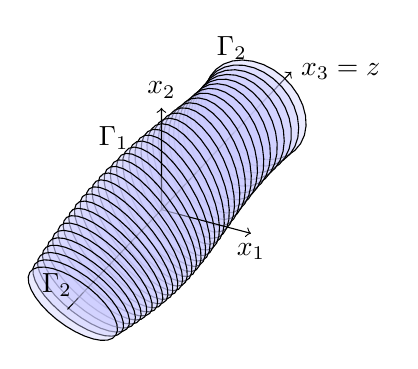
\begin{tikzpicture}[join=round,scale=0.6]
\draw[arrows=->,line width=.4pt](0,0)--(.758,.805);
\filldraw[fill=blue!20,fill opacity=0.4](.584,.697)--(.384,.847)--(.168,.959)--(-.056,1.029)--(-.277,1.055)--(-.487,1.034)--(-.675,.969)--(-.833,.86)--(-.955,.715)--(-1.036,.538)--(-1.071,.337)--(-1.059,.122)--(-1.001,-.099)--(-.899,-.315)--(-.758,-.517)--(-.584,-.697)--(-.384,-.847)--(-.168,-.959)--(.056,-1.029)--(.277,-1.055)--(.487,-1.034)--(.675,-.969)--(.833,-.86)--(.955,-.715)--(1.036,-.538)--(1.071,-.337)--(1.059,-.122)--(1.001,.099)--(.899,.315)--(.758,.517)--cycle;
\draw[arrows=-,line width=.4pt](-.114,-.121)--(0,0);
\filldraw[fill=blue!20,fill opacity=0.4](.38,.658)--(.181,.794)--(-.03,.89)--(-.245,.942)--(-.455,.948)--(-.649,.906)--(-.82,.82)--(-.96,.693)--(-1.064,.531)--(-1.125,.339)--(-1.143,.128)--(-1.115,-.094)--(-1.044,-.317)--(-.932,-.532)--(-.784,-.729)--(-.607,-.899)--(-.409,-1.035)--(-.197,-1.131)--(.018,-1.183)--(.227,-1.189)--(.422,-1.148)--(.593,-1.062)--(.733,-.935)--(.836,-.772)--(.898,-.581)--(.915,-.369)--(.888,-.147)--(.816,.076)--(.705,.291)--(.557,.488)--cycle;
\draw[arrows=-,line width=.4pt](-.227,-.241)--(-.114,-.121);
\filldraw[fill=blue!20,fill opacity=0.4](.175,.613)--(-.021,.735)--(-.227,.815)--(-.432,.849)--(-.629,.835)--(-.808,.774)--(-.961,.668)--(-1.083,.523)--(-1.167,.344)--(-1.21,.14)--(-1.211,-.081)--(-1.168,-.308)--(-1.084,-.533)--(-.962,-.746)--(-.809,-.936)--(-.63,-1.096)--(-.434,-1.218)--(-.228,-1.298)--(-.023,-1.331)--(.174,-1.317)--(.353,-1.256)--(.507,-1.151)--(.628,-1.006)--(.712,-.827)--(.756,-.623)--(.756,-.402)--(.713,-.174)--(.629,.051)--(.508,.263)--(.354,.453)--cycle;
\draw[arrows=-,line width=.4pt](-.341,-.362)--(-.227,-.241);
\filldraw[fill=blue!20,fill opacity=0.4](-.029,.562)--(-.223,.671)--(-.421,.734)--(-.617,.749)--(-.8,.716)--(-.963,.636)--(-1.099,.512)--(-1.201,.35)--(-1.267,.157)--(-1.291,-.059)--(-1.275,-.288)--(-1.217,-.52)--(-1.121,-.746)--(-.991,-.955)--(-.833,-1.137)--(-.653,-1.286)--(-.459,-1.395)--(-.261,-1.458)--(-.066,-1.474)--(.117,-1.44)--(.28,-1.36)--(.416,-1.236)--(.519,-1.074)--(.584,-.881)--(.609,-.665)--(.592,-.436)--(.535,-.204)--(.439,.022)--(.309,.23)--(.15,.413)--cycle;
\draw[arrows=-,line width=.4pt](-.455,-.483)--(-.341,-.362);
\filldraw[fill=blue!20,fill opacity=0.4](-.234,.505)--(-.423,.6)--(-.614,.647)--(-.798,.644)--(-.967,.593)--(-1.114,.494)--(-1.232,.353)--(-1.315,.175)--(-1.362,-.032)--(-1.368,-.258)--(-1.335,-.494)--(-1.263,-.73)--(-1.156,-.955)--(-1.018,-1.159)--(-.856,-1.333)--(-.676,-1.471)--(-.486,-1.565)--(-.296,-1.612)--(-.112,-1.61)--(.057,-1.558)--(.204,-1.46)--(.322,-1.318)--(.406,-1.14)--(.452,-.934)--(.459,-.707)--(.425,-.471)--(.354,-.236)--(.246,-.011)--(.109,.193)--(-.054,.368)--cycle;
\draw[arrows=-,line width=.4pt](-.569,-.603)--(-.455,-.483);
\filldraw[fill=blue!20,fill opacity=0.4](-.437,.443)--(-.622,.523)--(-.805,.553)--(-.977,.533)--(-1.131,.464)--(-1.261,.348)--(-1.36,.19)--(-1.425,-.003)--(-1.453,-.221)--(-1.442,-.457)--(-1.392,-.698)--(-1.307,-.936)--(-1.189,-1.159)--(-1.045,-1.358)--(-.879,-1.524)--(-.7,-1.65)--(-.515,-1.729)--(-.333,-1.76)--(-.16,-1.74)--(-.006,-1.671)--(.124,-1.555)--(.223,-1.397)--(.288,-1.204)--(.316,-.986)--(.304,-.75)--(.255,-.508)--(.17,-.271)--(.052,-.048)--(-.092,.151)--(-.258,.317)--cycle;
\draw[arrows=-,line width=.4pt](-.682,-.724)--(-.569,-.603);
\filldraw[fill=blue!20,fill opacity=0.4](-.639,.373)--(-.819,.439)--(-.992,.454)--(-1.152,.417)--(-1.291,.33)--(-1.404,.197)--(-1.485,.024)--(-1.531,-.182)--(-1.54,-.411)--(-1.512,-.654)--(-1.447,-.901)--(-1.349,-1.139)--(-1.221,-1.359)--(-1.07,-1.552)--(-.903,-1.708)--(-.725,-1.822)--(-.546,-1.887)--(-.373,-1.902)--(-.213,-1.865)--(-.073,-1.778)--(.039,-1.645)--(.12,-1.472)--(.166,-1.267)--(.175,-1.037)--(.147,-.794)--(.082,-.548)--(-.016,-.309)--(-.143,-.089)--(-.294,.104)--(-.462,.26)--cycle;
\draw[arrows=-,line width=.4pt](-.796,-.845)--(-.682,-.724);
\filldraw[fill=blue!20,fill opacity=0.4](-.84,.298)--(-1.013,.349)--(-1.177,.348)--(-1.323,.294)--(-1.447,.191)--(-1.543,.043)--(-1.605,-.144)--(-1.633,-.362)--(-1.624,-.601)--(-1.578,-.851)--(-1.499,-1.1)--(-1.388,-1.338)--(-1.252,-1.555)--(-1.096,-1.74)--(-.927,-1.887)--(-.752,-1.988)--(-.579,-2.039)--(-.415,-2.037)--(-.269,-1.984)--(-.145,-1.881)--(-.049,-1.732)--(.013,-1.545)--(.041,-1.327)--(.032,-1.088)--(-.014,-.839)--(-.093,-.59)--(-.204,-.351)--(-.34,-.135)--(-.496,.051)--(-.665,.197)--cycle;
\draw[arrows=-,line width=.4pt](-.91,-.966)--(-.796,-.845);
\filldraw[fill=blue!20,fill opacity=0.4](-1.039,.216)--(-1.205,.252)--(-1.358,.236)--(-1.491,.166)--(-1.599,.048)--(-1.677,-.115)--(-1.722,-.315)--(-1.731,-.544)--(-1.704,-.791)--(-1.642,-1.046)--(-1.548,-1.297)--(-1.427,-1.533)--(-1.283,-1.745)--(-1.122,-1.923)--(-.952,-2.059)--(-.781,-2.147)--(-.615,-2.183)--(-.462,-2.167)--(-.328,-2.097)--(-.22,-1.979)--(-.142,-1.816)--(-.098,-1.616)--(-.089,-1.387)--(-.116,-1.14)--(-.177,-.886)--(-.271,-.634)--(-.393,-.398)--(-.537,-.186)--(-.697,-.008)--(-.867,.128)--cycle;
\draw[arrows=-,line width=.4pt](-1.023,-1.086)--(-.91,-.966);
\filldraw[fill=blue!20,fill opacity=0.4](-1.235,.127)--(-1.393,.149)--(-1.535,.118)--(-1.655,.033)--(-1.747,-.1)--(-1.808,-.277)--(-1.834,-.488)--(-1.825,-.726)--(-1.781,-.98)--(-1.703,-1.238)--(-1.596,-1.49)--(-1.464,-1.724)--(-1.313,-1.93)--(-1.149,-2.099)--(-.98,-2.224)--(-.812,-2.3)--(-.654,-2.322)--(-.512,-2.29)--(-.392,-2.206)--(-.3,-2.072)--(-.239,-1.896)--(-.213,-1.684)--(-.222,-1.446)--(-.266,-1.192)--(-.343,-.934)--(-.45,-.682)--(-.582,-.448)--(-.734,-.242)--(-.898,-.073)--(-1.067,.052)--cycle;
\draw[arrows=-,line width=.4pt](-1.137,-1.207)--(-1.023,-1.086);
\filldraw[fill=blue!20,fill opacity=0.4](-1.428,.032)--(-1.578,.04)--(-1.709,-.006)--(-1.815,-.105)--(-1.891,-.252)--(-1.934,-.441)--(-1.943,-.663)--(-1.916,-.909)--(-1.855,-1.168)--(-1.763,-1.429)--(-1.643,-1.68)--(-1.501,-1.91)--(-1.344,-2.11)--(-1.177,-2.27)--(-1.009,-2.384)--(-.846,-2.446)--(-.696,-2.454)--(-.565,-2.407)--(-.459,-2.308)--(-.383,-2.161)--(-.34,-1.973)--(-.332,-1.75)--(-.359,-1.504)--(-.419,-1.245)--(-.512,-.985)--(-.631,-.734)--(-.773,-.504)--(-.931,-.304)--(-1.097,-.144)--(-1.266,-.03)--cycle;
\draw[arrows=-,line width=.4pt](-1.251,-1.328)--(-1.137,-1.207);
\filldraw[fill=blue!20,fill opacity=0.4](-1.619,-.07)--(-1.76,-.076)--(-1.879,-.136)--(-1.97,-.249)--(-2.03,-.409)--(-2.056,-.608)--(-2.047,-.84)--(-2.003,-1.092)--(-1.926,-1.355)--(-1.82,-1.617)--(-1.689,-1.866)--(-1.538,-2.092)--(-1.375,-2.284)--(-1.207,-2.434)--(-1.04,-2.536)--(-.883,-2.585)--(-.742,-2.579)--(-.623,-2.519)--(-.531,-2.406)--(-.471,-2.247)--(-.445,-2.047)--(-.455,-1.815)--(-.499,-1.563)--(-.576,-1.3)--(-.682,-1.038)--(-.813,-.789)--(-.964,-.563)--(-1.127,-.371)--(-1.295,-.221)--(-1.461,-.119)--cycle;
\draw[arrows=-,line width=.4pt](-1.365,-1.448)--(-1.251,-1.328);
\filldraw[fill=blue!20,fill opacity=0.4](-1.806,-.178)--(-1.937,-.198)--(-2.044,-.272)--(-2.121,-.397)--(-2.165,-.568)--(-2.174,-.778)--(-2.148,-1.017)--(-2.087,-1.275)--(-1.995,-1.541)--(-1.875,-1.802)--(-1.733,-2.048)--(-1.575,-2.268)--(-1.408,-2.452)--(-1.238,-2.592)--(-1.075,-2.682)--(-.924,-2.718)--(-.792,-2.699)--(-.685,-2.625)--(-.608,-2.499)--(-.564,-2.328)--(-.555,-2.118)--(-.581,-1.879)--(-.642,-1.621)--(-.734,-1.356)--(-.854,-1.094)--(-.996,-.848)--(-1.154,-.628)--(-1.321,-.444)--(-1.491,-.304)--(-1.655,-.214)--cycle;
\draw[arrows=-,line width=.4pt](-1.478,-1.569)--(-1.365,-1.448);
\filldraw[fill=blue!20,fill opacity=0.4](-1.989,-.293)--(-2.111,-.326)--(-2.205,-.412)--(-2.268,-.55)--(-2.296,-.732)--(-2.288,-.95)--(-2.245,-1.196)--(-2.169,-1.458)--(-2.062,-1.725)--(-1.93,-1.985)--(-1.778,-2.226)--(-1.613,-2.439)--(-1.442,-2.614)--(-1.272,-2.744)--(-1.112,-2.822)--(-.968,-2.845)--(-.846,-2.812)--(-.751,-2.725)--(-.689,-2.588)--(-.661,-2.406)--(-.668,-2.187)--(-.711,-1.942)--(-.788,-1.68)--(-.895,-1.413)--(-1.027,-1.153)--(-1.179,-.912)--(-1.344,-.699)--(-1.515,-.524)--(-1.684,-.394)--(-1.845,-.316)--cycle;
\draw[arrows=-,line width=.4pt](-1.592,-1.69)--(-1.478,-1.569);
\filldraw[fill=blue!20,fill opacity=0.4](-2.168,-.414)--(-2.28,-.46)--(-2.362,-.559)--(-2.41,-.707)--(-2.422,-.899)--(-2.398,-1.125)--(-2.339,-1.375)--(-2.247,-1.64)--(-2.127,-1.906)--(-1.983,-2.163)--(-1.822,-2.4)--(-1.651,-2.605)--(-1.478,-2.771)--(-1.309,-2.889)--(-1.153,-2.955)--(-1.016,-2.965)--(-.904,-2.92)--(-.822,-2.821)--(-.774,-2.672)--(-.762,-2.481)--(-.786,-2.255)--(-.845,-2.004)--(-.937,-1.74)--(-1.057,-1.473)--(-1.201,-1.216)--(-1.362,-.979)--(-1.533,-.774)--(-1.707,-.609)--(-1.875,-.49)--(-2.031,-.425)--cycle;
\draw[arrows=-,line width=.4pt](-1.706,-1.81)--(-1.592,-1.69);
\filldraw[fill=blue!20,fill opacity=0.4](-2.344,-.542)--(-2.445,-.599)--(-2.514,-.71)--(-2.547,-.868)--(-2.544,-1.068)--(-2.505,-1.3)--(-2.43,-1.555)--(-2.324,-1.82)--(-2.19,-2.086)--(-2.036,-2.339)--(-1.867,-2.569)--(-1.691,-2.766)--(-1.516,-2.921)--(-1.348,-3.028)--(-1.197,-3.081)--(-1.068,-3.079)--(-.967,-3.022)--(-.898,-2.911)--(-.864,-2.752)--(-.867,-2.553)--(-.907,-2.32)--(-.982,-2.066)--(-1.088,-1.8)--(-1.221,-1.535)--(-1.376,-1.282)--(-1.545,-1.052)--(-1.721,-.855)--(-1.896,-.7)--(-2.063,-.593)--(-2.214,-.54)--cycle;
\draw[arrows=-,line width=.4pt](-1.819,-1.931)--(-1.706,-1.81);
\filldraw[fill=blue!20,fill opacity=0.4](-2.514,-.675)--(-2.605,-.744)--(-2.661,-.866)--(-2.68,-1.033)--(-2.662,-1.24)--(-2.607,-1.477)--(-2.518,-1.734)--(-2.398,-2)--(-2.252,-2.262)--(-2.088,-2.51)--(-1.912,-2.733)--(-1.732,-2.921)--(-1.556,-3.065)--(-1.391,-3.16)--(-1.245,-3.201)--(-1.125,-3.187)--(-1.034,-3.118)--(-.978,-2.997)--(-.959,-2.829)--(-.977,-2.622)--(-1.032,-2.385)--(-1.121,-2.128)--(-1.241,-1.862)--(-1.387,-1.6)--(-1.551,-1.352)--(-1.727,-1.129)--(-1.907,-.941)--(-2.083,-.797)--(-2.248,-.702)--(-2.393,-.661)--cycle;
\draw[arrows=-,line width=.4pt](-1.933,-2.052)--(-1.819,-1.931);
\filldraw[fill=blue!20,fill opacity=0.4](-2.681,-.814)--(-2.76,-.895)--(-2.803,-1.026)--(-2.809,-1.202)--(-2.776,-1.415)--(-2.706,-1.655)--(-2.602,-1.914)--(-2.469,-2.178)--(-2.313,-2.436)--(-2.14,-2.678)--(-1.958,-2.893)--(-1.775,-3.07)--(-1.599,-3.204)--(-1.438,-3.286)--(-1.298,-3.315)--(-1.186,-3.289)--(-1.106,-3.209)--(-1.063,-3.078)--(-1.058,-2.902)--(-1.091,-2.689)--(-1.16,-2.448)--(-1.264,-2.19)--(-1.397,-1.926)--(-1.553,-1.667)--(-1.726,-1.425)--(-1.908,-1.211)--(-2.091,-1.033)--(-2.267,-.9)--(-2.428,-.817)--(-2.568,-.788)--cycle;
\draw[arrows=-,line width=.4pt](-2.047,-2.172)--(-1.933,-2.052);
\draw[arrows=<->,line width=.4pt](-.095,-2.615)--(-1.99,-2.112)--(-1.99,.043);
\filldraw[fill=blue!20,fill opacity=0.4](-2.842,-.959)--(-2.91,-1.05)--(-2.941,-1.19)--(-2.932,-1.373)--(-2.885,-1.591)--(-2.801,-1.834)--(-2.684,-2.092)--(-2.54,-2.354)--(-2.373,-2.607)--(-2.193,-2.842)--(-2.006,-3.047)--(-1.821,-3.214)--(-1.646,-3.336)--(-1.488,-3.407)--(-1.355,-3.423)--(-1.252,-3.385)--(-1.183,-3.294)--(-1.153,-3.155)--(-1.161,-2.972)--(-1.209,-2.754)--(-1.293,-2.511)--(-1.409,-2.253)--(-1.554,-1.991)--(-1.72,-1.737)--(-1.901,-1.503)--(-2.088,-1.298)--(-2.273,-1.13)--(-2.448,-1.009)--(-2.606,-.938)--(-2.739,-.921)--cycle;
\draw[arrows=-,line width=.4pt](-2.161,-2.293)--(-2.047,-2.172);
\filldraw[fill=blue!20,fill opacity=0.4](-2.999,-1.11)--(-3.056,-1.211)--(-3.073,-1.359)--(-3.051,-1.548)--(-2.99,-1.769)--(-2.893,-2.014)--(-2.764,-2.27)--(-2.608,-2.528)--(-2.433,-2.775)--(-2.246,-3.002)--(-2.055,-3.197)--(-1.869,-3.353)--(-1.696,-3.462)--(-1.542,-3.521)--(-1.416,-3.525)--(-1.323,-3.476)--(-1.266,-3.376)--(-1.248,-3.228)--(-1.27,-3.039)--(-1.331,-2.817)--(-1.428,-2.573)--(-1.557,-2.316)--(-1.713,-2.058)--(-1.888,-1.811)--(-2.075,-1.585)--(-2.266,-1.389)--(-2.452,-1.233)--(-2.626,-1.124)--(-2.779,-1.066)--(-2.905,-1.061)--cycle;
\draw[arrows=-,line width=.4pt](-2.274,-2.414)--(-2.161,-2.293);
\filldraw[fill=blue!20,fill opacity=0.4](-3.15,-1.265)--(-3.196,-1.375)--(-3.201,-1.531)--(-3.166,-1.725)--(-3.092,-1.949)--(-2.982,-2.193)--(-2.841,-2.447)--(-2.676,-2.7)--(-2.493,-2.94)--(-2.3,-3.157)--(-2.106,-3.341)--(-1.92,-3.486)--(-1.749,-3.583)--(-1.601,-3.629)--(-1.482,-3.622)--(-1.398,-3.562)--(-1.353,-3.452)--(-1.347,-3.297)--(-1.382,-3.103)--(-1.457,-2.879)--(-1.566,-2.635)--(-1.707,-2.381)--(-1.873,-2.128)--(-2.056,-1.888)--(-2.249,-1.671)--(-2.442,-1.486)--(-2.629,-1.342)--(-2.8,-1.245)--(-2.948,-1.199)--(-3.066,-1.206)--cycle;
\draw[arrows=-,line width=.4pt](-2.388,-2.534)--(-2.274,-2.414);
\filldraw[fill=blue!20,fill opacity=0.4](-3.297,-1.426)--(-3.331,-1.544)--(-3.324,-1.706)--(-3.276,-1.904)--(-3.19,-2.129)--(-3.068,-2.372)--(-2.917,-2.623)--(-2.742,-2.869)--(-2.552,-3.101)--(-2.355,-3.308)--(-2.159,-3.481)--(-1.974,-3.613)--(-1.806,-3.698)--(-1.664,-3.731)--(-1.553,-3.713)--(-1.479,-3.643)--(-1.445,-3.525)--(-1.452,-3.363)--(-1.5,-3.165)--(-1.586,-2.94)--(-1.708,-2.697)--(-1.859,-2.446)--(-2.034,-2.2)--(-2.224,-1.968)--(-2.421,-1.761)--(-2.617,-1.588)--(-2.802,-1.456)--(-2.97,-1.371)--(-3.112,-1.337)--(-3.223,-1.356)--cycle;
\draw[arrows=-,line width=.4pt](-2.502,-2.655)--(-2.388,-2.534);
\filldraw[fill=blue!20,fill opacity=0.4](-3.438,-1.591)--(-3.461,-1.717)--(-3.442,-1.884)--(-3.382,-2.085)--(-3.284,-2.31)--(-3.151,-2.551)--(-2.99,-2.796)--(-2.808,-3.036)--(-2.612,-3.258)--(-2.412,-3.454)--(-2.215,-3.615)--(-2.031,-3.735)--(-1.867,-3.807)--(-1.732,-3.829)--(-1.629,-3.799)--(-1.565,-3.719)--(-1.542,-3.593)--(-1.561,-3.426)--(-1.621,-3.226)--(-1.719,-3)--(-1.852,-2.759)--(-2.013,-2.514)--(-2.195,-2.275)--(-2.391,-2.052)--(-2.592,-1.856)--(-2.788,-1.695)--(-2.973,-1.576)--(-3.136,-1.504)--(-3.272,-1.482)--(-3.374,-1.511)--cycle;
\draw[arrows=-,line width=.4pt](-2.615,-2.776)--(-2.502,-2.655);
\filldraw[fill=blue!20,fill opacity=0.4](-3.574,-1.76)--(-3.586,-1.893)--(-3.556,-2.065)--(-3.484,-2.267)--(-3.375,-2.492)--(-3.232,-2.729)--(-3.062,-2.969)--(-2.873,-3.199)--(-2.673,-3.412)--(-2.47,-3.596)--(-2.273,-3.745)--(-2.091,-3.851)--(-1.933,-3.911)--(-1.804,-3.92)--(-1.71,-3.88)--(-1.656,-3.792)--(-1.645,-3.659)--(-1.675,-3.487)--(-1.747,-3.284)--(-1.856,-3.06)--(-1.999,-2.822)--(-2.168,-2.583)--(-2.358,-2.352)--(-2.558,-2.14)--(-2.761,-1.955)--(-2.958,-1.807)--(-3.139,-1.7)--(-3.298,-1.641)--(-3.427,-1.631)--(-3.521,-1.672)--cycle;
\draw[arrows=-,line width=.4pt](-2.729,-2.897)--(-2.615,-2.776);
\filldraw[fill=blue!20,fill opacity=0.4](-3.705,-1.933)--(-3.707,-2.073)--(-3.665,-2.248)--(-3.582,-2.451)--(-3.462,-2.674)--(-3.31,-2.907)--(-3.133,-3.139)--(-2.938,-3.36)--(-2.734,-3.562)--(-2.53,-3.734)--(-2.334,-3.87)--(-2.156,-3.963)--(-2.002,-4.009)--(-1.881,-4.007)--(-1.796,-3.957)--(-1.753,-3.86)--(-1.752,-3.721)--(-1.793,-3.546)--(-1.876,-3.342)--(-1.996,-3.119)--(-2.148,-2.887)--(-2.325,-2.654)--(-2.52,-2.433)--(-2.724,-2.231)--(-2.929,-2.059)--(-3.124,-1.923)--(-3.303,-1.83)--(-3.456,-1.784)--(-3.577,-1.786)--(-3.662,-1.836)--cycle;
\draw[arrows=-,line width=.4pt](-2.843,-3.017)--(-2.729,-2.897);
\filldraw[fill=blue!20,fill opacity=0.4](-3.831,-2.11)--(-3.822,-2.255)--(-3.769,-2.432)--(-3.676,-2.636)--(-3.547,-2.856)--(-3.387,-3.083)--(-3.203,-3.307)--(-3.003,-3.518)--(-2.796,-3.708)--(-2.592,-3.867)--(-2.398,-3.989)--(-2.224,-4.069)--(-2.077,-4.103)--(-1.963,-4.089)--(-1.888,-4.029)--(-1.854,-3.924)--(-1.864,-3.78)--(-1.916,-3.602)--(-2.009,-3.399)--(-2.139,-3.179)--(-2.299,-2.952)--(-2.483,-2.728)--(-2.683,-2.516)--(-2.889,-2.327)--(-3.094,-2.167)--(-3.288,-2.045)--(-3.462,-1.965)--(-3.609,-1.931)--(-3.723,-1.945)--(-3.798,-2.006)--cycle;
\draw[arrows=-,line width=.4pt](-2.957,-3.138)--(-2.843,-3.017);
\filldraw[fill=blue!20,fill opacity=0.4](-3.952,-2.29)--(-3.932,-2.439)--(-3.869,-2.619)--(-3.767,-2.821)--(-3.629,-3.037)--(-3.461,-3.257)--(-3.272,-3.472)--(-3.068,-3.673)--(-2.86,-3.85)--(-2.656,-3.996)--(-2.465,-4.104)--(-2.296,-4.171)--(-2.155,-4.192)--(-2.05,-4.167)--(-1.984,-4.097)--(-1.961,-3.985)--(-1.981,-3.837)--(-2.044,-3.657)--(-2.146,-3.455)--(-2.285,-3.239)--(-2.452,-3.019)--(-2.642,-2.804)--(-2.845,-2.603)--(-3.053,-2.426)--(-3.257,-2.28)--(-3.448,-2.171)--(-3.617,-2.105)--(-3.758,-2.084)--(-3.863,-2.109)--(-3.929,-2.179)--cycle;
\draw[arrows=-,line width=.4pt](-3.07,-3.259)--(-2.957,-3.138);
\filldraw[fill=blue!20,fill opacity=0.4](-4.068,-2.474)--(-4.038,-2.626)--(-3.965,-2.806)--(-3.854,-3.006)--(-3.708,-3.217)--(-3.534,-3.43)--(-3.34,-3.635)--(-3.134,-3.824)--(-2.925,-3.988)--(-2.723,-4.12)--(-2.536,-4.215)--(-2.372,-4.268)--(-2.239,-4.276)--(-2.142,-4.241)--(-2.086,-4.162)--(-2.072,-4.044)--(-2.103,-3.891)--(-2.175,-3.711)--(-2.287,-3.511)--(-2.433,-3.3)--(-2.607,-3.087)--(-2.801,-2.882)--(-3.007,-2.693)--(-3.215,-2.529)--(-3.418,-2.397)--(-3.605,-2.302)--(-3.768,-2.25)--(-3.902,-2.241)--(-3.999,-2.277)--(-4.055,-2.355)--cycle;
\draw[arrows=-,line width=.4pt](-3.184,-3.379)--(-3.07,-3.259);
\filldraw[fill=blue!20,fill opacity=0.4](-4.179,-2.659)--(-4.139,-2.814)--(-4.057,-2.994)--(-3.937,-3.191)--(-3.784,-3.396)--(-3.605,-3.601)--(-3.408,-3.795)--(-3.2,-3.972)--(-2.992,-4.122)--(-2.793,-4.24)--(-2.61,-4.321)--(-2.452,-4.36)--(-2.327,-4.357)--(-2.239,-4.31)--(-2.192,-4.223)--(-2.189,-4.1)--(-2.229,-3.944)--(-2.311,-3.764)--(-2.431,-3.567)--(-2.584,-3.362)--(-2.763,-3.158)--(-2.96,-2.963)--(-3.168,-2.787)--(-3.376,-2.636)--(-3.576,-2.518)--(-3.758,-2.438)--(-3.916,-2.398)--(-4.041,-2.402)--(-4.129,-2.448)--(-4.176,-2.535)--cycle;
\draw[arrows=-,line width=.4pt](-3.298,-3.5)--(-3.184,-3.379);
\filldraw[fill=blue!20,fill opacity=0.4](-4.285,-2.847)--(-4.236,-3.004)--(-4.145,-3.183)--(-4.018,-3.376)--(-3.859,-3.574)--(-3.675,-3.769)--(-3.475,-3.953)--(-3.267,-4.116)--(-3.061,-4.253)--(-2.865,-4.356)--(-2.688,-4.423)--(-2.537,-4.449)--(-2.42,-4.433)--(-2.341,-4.377)--(-2.304,-4.282)--(-2.31,-4.153)--(-2.36,-3.996)--(-2.45,-3.817)--(-2.578,-3.624)--(-2.737,-3.426)--(-2.92,-3.231)--(-3.12,-3.047)--(-3.328,-2.884)--(-3.534,-2.747)--(-3.731,-2.644)--(-3.908,-2.577)--(-4.058,-2.551)--(-4.176,-2.567)--(-4.255,-2.623)--(-4.292,-2.718)--cycle;
\draw[arrows=-,line width=.4pt](-3.411,-3.621)--(-3.298,-3.5);
\filldraw[fill=blue!20,fill opacity=0.4](-4.387,-3.036)--(-4.328,-3.195)--(-4.23,-3.372)--(-4.096,-3.56)--(-3.931,-3.751)--(-3.745,-3.936)--(-3.543,-4.107)--(-3.336,-4.257)--(-3.132,-4.379)--(-2.94,-4.468)--(-2.769,-4.52)--(-2.626,-4.533)--(-2.517,-4.506)--(-2.448,-4.44)--(-2.42,-4.338)--(-2.436,-4.205)--(-2.494,-4.046)--(-2.593,-3.869)--(-2.727,-3.681)--(-2.891,-3.49)--(-3.078,-3.305)--(-3.28,-3.134)--(-3.487,-2.984)--(-3.691,-2.862)--(-3.883,-2.773)--(-4.054,-2.721)--(-4.197,-2.709)--(-4.306,-2.736)--(-4.375,-2.802)--(-4.403,-2.903)--cycle;
\draw[arrows=-,line width=.4pt](-3.525,-3.741)--(-3.411,-3.621);
\filldraw[fill=blue!20,fill opacity=0.4](-4.484,-3.227)--(-4.417,-3.386)--(-4.311,-3.561)--(-4.171,-3.743)--(-4.002,-3.926)--(-3.813,-4.1)--(-3.611,-4.258)--(-3.405,-4.394)--(-3.205,-4.502)--(-3.019,-4.576)--(-2.854,-4.614)--(-2.719,-4.614)--(-2.62,-4.575)--(-2.559,-4.5)--(-2.541,-4.392)--(-2.566,-4.255)--(-2.633,-4.096)--(-2.739,-3.922)--(-2.88,-3.739)--(-3.048,-3.557)--(-3.237,-3.383)--(-3.439,-3.224)--(-3.645,-3.088)--(-3.845,-2.981)--(-4.032,-2.907)--(-4.196,-2.869)--(-4.331,-2.869)--(-4.431,-2.908)--(-4.491,-2.983)--(-4.509,-3.091)--cycle;
\draw[arrows=-,line width=.4pt](-3.639,-3.862)--(-3.525,-3.741);
\filldraw[fill=blue!20,fill opacity=0.4](-4.576,-3.419)--(-4.502,-3.578)--(-4.389,-3.749)--(-4.244,-3.925)--(-4.072,-4.098)--(-3.881,-4.261)--(-3.68,-4.407)--(-3.477,-4.528)--(-3.281,-4.621)--(-3.1,-4.68)--(-2.943,-4.704)--(-2.817,-4.691)--(-2.727,-4.641)--(-2.676,-4.558)--(-2.667,-4.444)--(-2.701,-4.305)--(-2.776,-4.146)--(-2.889,-3.975)--(-3.034,-3.799)--(-3.206,-3.626)--(-3.397,-3.463)--(-3.598,-3.317)--(-3.801,-3.196)--(-3.997,-3.103)--(-4.177,-3.044)--(-4.334,-3.02)--(-4.461,-3.033)--(-4.551,-3.083)--(-4.602,-3.166)--(-4.61,-3.28)--cycle;
\draw[arrows=-,line width=.4pt](-3.753,-3.983)--(-3.639,-3.862);
\filldraw[fill=blue!20,fill opacity=0.4](-4.665,-3.612)--(-4.583,-3.77)--(-4.464,-3.936)--(-4.314,-4.105)--(-4.14,-4.269)--(-3.949,-4.42)--(-3.749,-4.552)--(-3.549,-4.659)--(-3.359,-4.736)--(-3.185,-4.781)--(-3.036,-4.79)--(-2.919,-4.765)--(-2.838,-4.705)--(-2.797,-4.614)--(-2.798,-4.495)--(-2.84,-4.353)--(-2.923,-4.196)--(-3.041,-4.029)--(-3.191,-3.86)--(-3.365,-3.697)--(-3.556,-3.546)--(-3.756,-3.414)--(-3.956,-3.307)--(-4.146,-3.229)--(-4.32,-3.185)--(-4.469,-3.175)--(-4.586,-3.201)--(-4.667,-3.261)--(-4.708,-3.352)--(-4.707,-3.471)--cycle;
\draw[arrows=-,line width=.4pt](-3.866,-4.103)--(-3.753,-3.983);
\filldraw[fill=blue!20,fill opacity=0.4](-4.75,-3.805)--(-4.66,-3.961)--(-4.536,-4.123)--(-4.383,-4.284)--(-4.207,-4.437)--(-4.017,-4.575)--(-3.819,-4.693)--(-3.624,-4.785)--(-3.44,-4.848)--(-3.274,-4.878)--(-3.133,-4.874)--(-3.025,-4.836)--(-2.954,-4.766)--(-2.923,-4.668)--(-2.932,-4.544)--(-2.983,-4.402)--(-3.072,-4.246)--(-3.196,-4.084)--(-3.349,-3.923)--(-3.525,-3.77)--(-3.716,-3.632)--(-3.913,-3.514)--(-4.108,-3.421)--(-4.293,-3.359)--(-4.459,-3.329)--(-4.599,-3.333)--(-4.707,-3.371)--(-4.779,-3.441)--(-4.81,-3.539)--(-4.8,-3.663)--cycle;
\draw[arrows=-,line width=.4pt](-3.98,-4.224)--(-3.866,-4.103);
\path (.758,.805) node[right] {$x_3 = z$}
                   (-.095,-2.615) node[below] {$x_1$}
                   (-1.99,.043) node[above] {$x_2$};


\node at (-4.2,-3.7) {$\Gamma_2$};
\node at (-3.0,-0.6) {$\Gamma_1$};
\node at (-0.5, 1.3) {$\Gamma_2$};
\end{tikzpicture}% End sketch output
 \\
            \end{center}
            \vspace{0.2cm} 
			$\Gamma_1$ is the surface of an
    		\begin{enumerate}
	    		\item elliptic beam-pipe
		    	\item arbitrary beam-pipe element
    		\end{enumerate}
		\end{column}
		\end{columns}
		
	\end{frame}

    \begin{frame}
    \frametitle{Extrapolation at Boundary}

        \begin{center}
            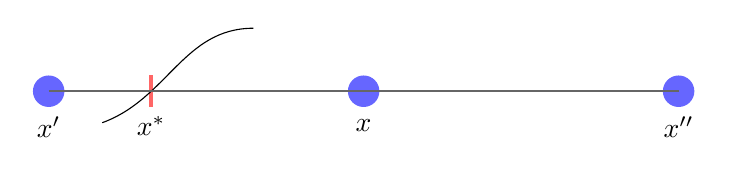
\begin{tikzpicture}
                \node [coordinate] at (-4,0) (xp) {};
                \fill[color=blue!60] (xp) circle (0.2);
                \node [coordinate] at (0,0) (x) {};
                \node at (-4,-0.2) [below] {$x'$};
                \fill[color=blue!60] (x) circle (0.2);
                \node [coordinate] at (4,0) (xpp) {};
                \node at (0,-0.24) [below] {$x$};
                \fill[color=blue!60] (xpp) circle (0.2);
                \node at (4,-0.2) [below] {$x''$};
                
                \node [coordinate] at (-2.7,0) (xs) {};
                \draw[very thick,rounded corners=8pt,color=red!60] (-2.7,-0.2) -- (-2.7,0.2);
                \draw (-3.32,-0.4) to[out=20,in=180] node [sloped,below] {} (-1.4,0.8);
                \node at (-2.7,-0.2) [below] {$x^*$};
                %\node at (-2.75,0.2) [above] {$x-sh$};

                \path[-,thick,color=black!60]<1-> (xp) edge (x);
                \path[-,thick,color=black!60]<1-> (x) edge (xpp);

            \end{tikzpicture}
        \end{center}
        \vspace{0.2cm}

        \begin{enumerate}
            %\item {\color{blue!60}\emph{Constant extrapolation}}: the boundary value prescribed at
                %$x^* \in \Gamma_1$ is assigned to $u(x')$
            \item {\color{blue!60}\emph{Constant extrapolation}}: $u(x') = u(x^*)$ and $x^* \in \Gamma_1$ 

            \item {\color{blue!60}\emph{Linear extrapolation}}: $u(x')$ is obtained by means of $u(x)$ and $u(x^*)$

            \item {\color{blue!60}\emph{Quadratic extrapolation}} (Shortley-Weller
                approximation): $u(x')$ is obtained by quadratic interpolation of $u(x)$, $u(x'')$, and $u(x^*)$\\
                $\rightarrow$ \alert{non-symmetric} stencil
        \end{enumerate}

    \end{frame}
    	
	

     \section{Results}

     	\begin{frame}
		\frametitle{Environment}

		\begin{exampleblock}{Buin: Cray XT4 cluster at the CSCS in Manno (Switzerland)}
		\begin{itemize}
			\item 468 AMD dual core Opteron at 2.6 GHz
			\item 936 GB DDR RAM
			\item 30 TB Disk
			\item 7.6 GB/s interconnect bandwith
		\end{itemize}
		\end{exampleblock}

		\begin{center}
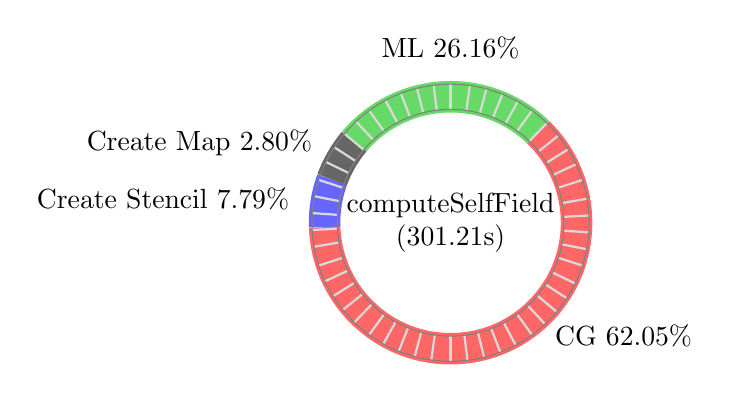
\begin{tikzpicture}[scale=0.8]
  \colorlet{CRSTENCIL}{blue!60!white}
  \colorlet{ML}{green!75!black!60!white}
  \colorlet{CG}{red!60!white}
  \colorlet{RECALCMAP}{black!60}

  \node[text centered,text width=3cm]{computeSelfField (301.21s)};

  \begin{scope}[line width=4mm,rotate=270]
    \draw[CRSTENCIL]	(-110:2cm) arc (-110:-88:2cm);
    \draw[CG]	        (-88:2cm) arc (-88:136:2cm);
    \draw[ML]           (136:2cm)  arc (136:230:2cm);
    \draw[RECALCMAP]	(230:2cm) arc (230:250:2cm);

    \newcount\mycount
    \foreach \angle in {0,72,...,3599}
    {
      \mycount=\angle\relax
      \divide\mycount by 10\relax
      \draw[black!15,thick] (\the\mycount:18mm) -- (\the\mycount:22mm);
    }
    
    \draw (180:2.2cm) node[above] {ML 26.16\%};
    \draw (-100:2.2cm) node[left] {Create Stencil 7.79\%};
    \draw (-125:2.2cm) node[left] {Create Map 2.80\%};
    \draw (35:2.2cm) node[right] {CG 62.05\%};
  \end{scope}  
  \draw[gray] (0,0) circle (2.2cm) circle (1.8cm);
\end{tikzpicture}
		\end{center}

	\end{frame}

     	\begin{frame}
		\frametitle{Validation of the Solver}

		For validation purposes we investigated an axi-symmetric potential function with known analytical solution. 

    	\begin{center}
	    \rowcolors{1}{blue!20}{blue!5}
        \begin{tabular}{lllll}
              \hline
              $h$ & $\vert\vert e_h \vert\vert_2$ & $r$ & $\vert\vert e_h
              \vert\vert_\infty$ & $r$ \\ [0.2ex] \hline \hline
              $1/64$  & $2.162 \times 10^{-3}$ & --- & $7.647 \times 10^{-3}$ & --- \\ 
              $1/128$ & $1.240 \times 10^{-3}$ & 0.80 & $4.153 \times 10^{-3}$ & 0.88 \\ 
              \hline
              \hline
              $1/64$  & $2.460 \times 10^{-5}$ & --- & $6.020 \times 10^{-5}$ & --- \\
              $1/128$ & $6.226 \times 10^{-6}$ & 1.98 & $1.437 \times 10^{-5}$ & 2.07 \\
              \hline
              \hline
              $1/64$  & $5.581 \times 10^{-6}$ & --- & $1.689 \times 10^{-5}$ & --- \\ 
              $1/128$ & $1.384 \times 10^{-7}$ & 2.01 & $4.550 \times 10^{-6}$ & 1.89  \\ 
            \hline
        \end{tabular}

        \vspace{0.2cm}
        \tiny{Solution error for constant (top), linear (middle)m quadratic (bottom) extrapolation}
        \end{center}

        \vspace{0.1cm}

        The convergence rate $r$ is defined by
        \[
            r = \log_2 \left( \frac{\vert\vert e_{2h} \vert\vert}{\vert\vert e_h \vert\vert} \right)
        \]
        and the convergence criterion
        \[
            \frac{\vert\vert r_k \vert\vert_2}{\vert\vert b \vert\vert_2} < \varepsilon = 10^{-6}
        \]

	\end{frame}
    
    \begin{frame}
        \frametitle{FFT vs. PCG}

        Simulation timings of one solve in the first and second time step, respectively

        \begin{center}
          \rowcolors{1}{blue!20}{blue!5}
          \begin{tabular}{cccccc}
            \hline
            solver & reusing & mesh size & mesh points & first [s] & second [s] \\
            \hline
            FFT & --- & $128\times128\times256$ & 4,194,304 & 12.3 & --- \\
            \hline
            PCG & --- & $128\times128\times256$ & 3,236,864 & 49.9 & 42.2 \\
            PCG & hier & $128\times128\times256$ & 3,236,864 & --- & 35.5 \\
            PCG & prec & $128\times128\times256$ & 3,236,864 & --- & 28.2 \\
            \hline
            PCG & --- & $166\times166\times256$ & 5,462,016 & 81.8 & 71.2 \\
            PCG & hier & $166\times166\times256$ & 5,462,016 & --- & 60.4 \\
            PCG & prec & $166\times166\times256$ & 5,462,016 & --- & 43.8 \\
            \hline
          \end{tabular}

          \vspace{0.2cm}
          \tiny{Equal number of mesh points (above) and equal mesh spacings (below) for FFT and AMG}
        \end{center}

        \vspace{0.1cm}

        \begin{itemize}
            \item Price we pay for increasing the accuracy of the simulation is approximately a {\color{red!60}factor of 2.5 -- 5}
        \end{itemize}

    \end{frame}

	\begin{frame}
		\frametitle{Parallel Efficiency}
		
		\begin{columns}
		\begin{column}{6.5cm}
            \centering
		        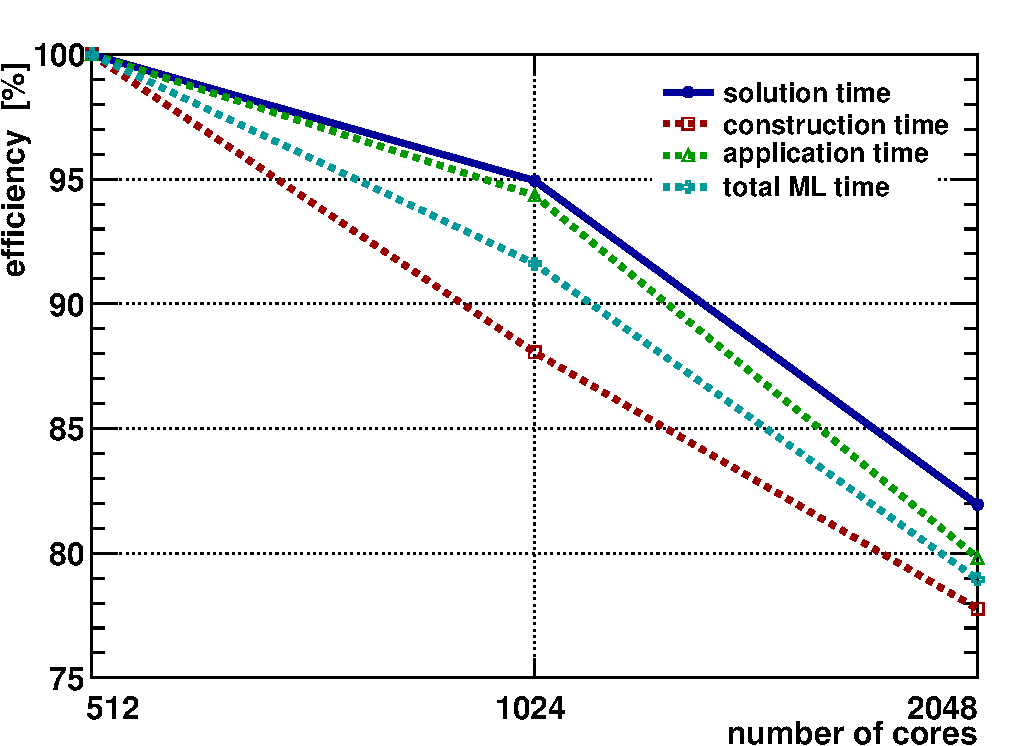
\includegraphics[width=0.99\textwidth]{plots/eff_1024_lin-crop.pdf}
        \end{column}
        \begin{column}{4.5cm}
            \begin{itemize} 
                \item Obtained for a tube embedded in a $1024\times1024\times1024$ grid
                \item Construction phase is performing the worst with an efficiency of 73\%
                \item Influence of problem size on the low performance of the aggregation in ML
            \end{itemize}
        \end{column}
        \end{columns}

	\end{frame}
	
    \begin{frame}
		\frametitle{Impact on Physics of \opal Simulations}
	
		\begin{columns}
		\begin{column}{6.5cm}
            \centering
		    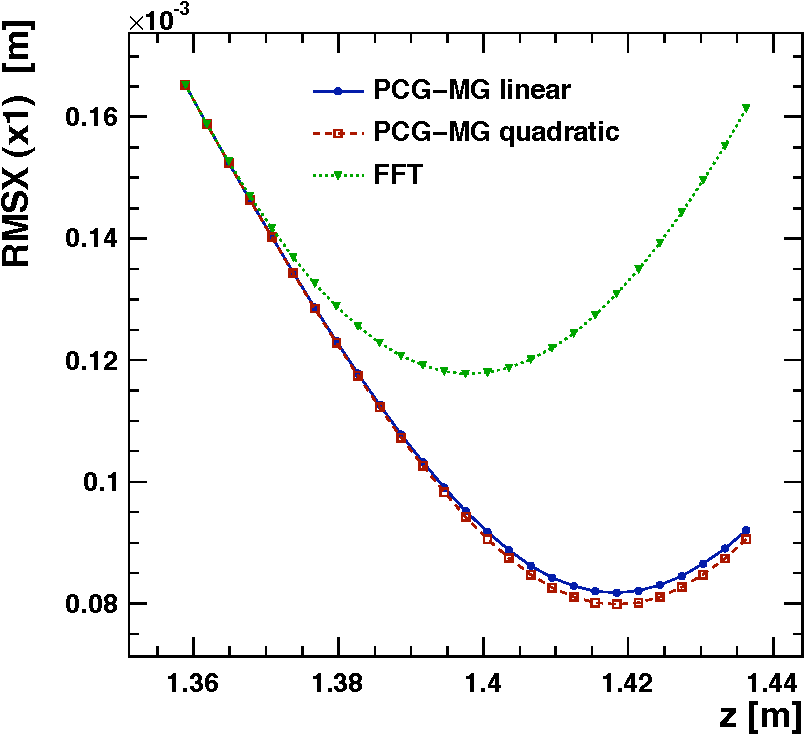
\includegraphics[width=0.99\textwidth]{plots/fft-drift-mg-drift-small-RMSX-x-SPOS-crop.pdf}
        \end{column}
        \begin{column}{4.5cm}
            \begin{itemize} 
                \item Statictics of the distance of the particle to the $z$-axis
                \item Shift of the beam size minimum (waist) towards larger $z$ values
                \item A {\color{red!60}smaller minimum} $\rightarrow$ self forces are larger when considering the beam pipe
                \item Beam pipe radius is an important optimization quantity
            \end{itemize}
        \end{column}
        \end{columns}

	\end{frame}
    
    \begin{frame}
        \frametitle{Load balance issue (1/2)}

		\begin{columns}
		\begin{column}{6.0cm}
            \centering
		    \includegraphics<1>[width=0.99\textwidth]{plots/dist_1_rect.png}
		    \includegraphics<2>[width=0.99\textwidth]{plots/dist_1.png}

            \vspace{0.1cm}
            \tiny{Cross section of data redistribution on $512$ cores on a $256 \times 256 \times 256$ grid (colors indicate data owned by a processor)}
        \end{column}
        \begin{column}{5.0cm}
            \begin{itemize} 
                \item Data distributed according to underlaying rectangular grid
                \item Load imbalance (some processors have nothing to do)
                \item However the work of the most heavily loaded core decreases linearly with the number of processors
                \item<2> Redistribute data with {\color{blue!60}recursive coordinate bisection (RCB)}
            \end{itemize}
        \end{column}
        \end{columns}

    \end{frame}

    \begin{frame}
        \frametitle{Load balance issue (2/2)}

		\begin{columns}
		\begin{column}{6.5cm}
            \centering
		    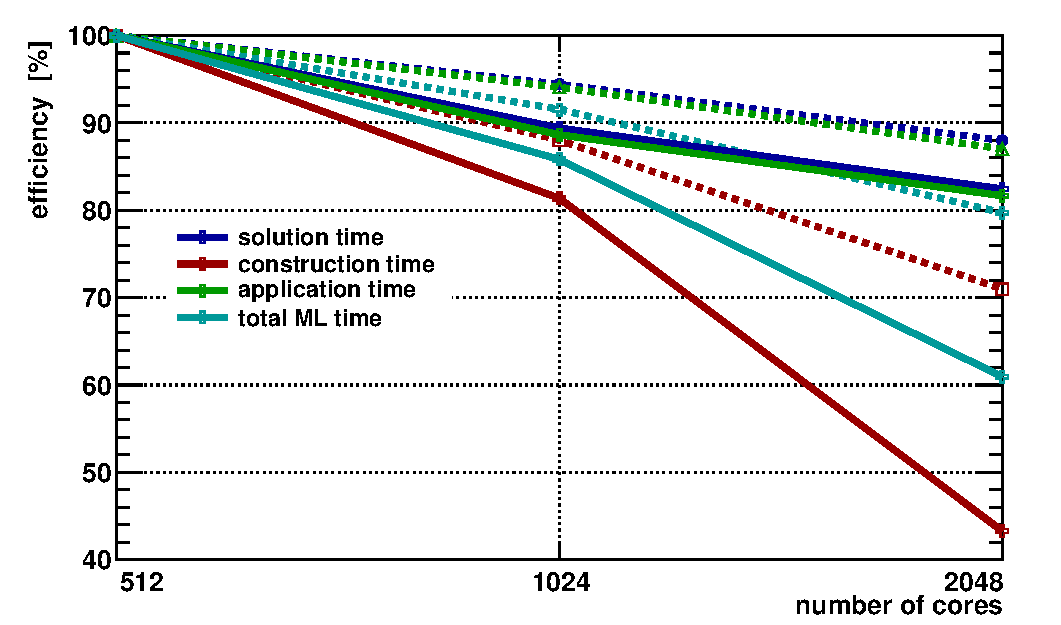
\includegraphics[width=0.99\textwidth]{plots/eff_new_1024.pdf}

        \end{column}
        \begin{column}{4.5cm}
            \begin{itemize} 
                \item Easier to get nice speedups for slow programms
                \item Unfair to start with both distributions at 100\% efficient (-$\pi/4$ ca 80\%)
                \item RCB distribution introduces more neighbours %starts to show when increasing the number of cores (more communication)
                \item Runtime for RCB better when communication is less penalizing
                \item Timing variations due to varying distribution of MPI tasks to processors?
            \end{itemize}
        \end{column}
        \end{columns}

    \end{frame}


    \section{Summary}

    \begin{frame}
		\frametitle{Summary}

		\begin{itemize}
			\item Conjugate gradient solver for Poisson equation on rectangular grid with special treatment of irregular boundary
			\item Elliptic and arbitrary domains based on real geometries
			\item Smoothed aggregation based algebraic Multigrid preconditioned CG
            \item Non-symmetric equations resulting from quadratic boundary treatment converge well with PCG
            \item Reducing time to solution (20 and 40\%) by reusing hierarchy or preconditioner
            \item Attaining good parallel efficiency: 73\% for the worst performing phase
            \item Compared to FFT more flexibilities for only a small performance loss
            \item Considerable impact on physics (e.g. for narrow beam pipes)
		\end{itemize}

    \end{frame}

    \begin{frame}
        \frametitle{Further Work}

		\begin{itemize}
			\item Validation of arbitrary domains against complex geometries
			\item Adaptive mesh refinement (AMR)
            \item Overcome Trilinos global index 32 bit integer size limitation
		\end{itemize}

	\end{frame}

%DONT COUNT BACKUP SLIDES
\addtocounter{framenumber}{-18}
\setbeamertemplate{footline}[default]

	\begin{frame}
	  	\frametitle{Backup}
		\begin{center}
			\color{blue}{\LARGE{Backup}}
		\end{center}
	\end{frame}
    
    \begin{frame}
        \frametitle{\opal in a Nutshell}

        \begin{alertblock}{}  
         \opal is a tool for charged-particle optics in large
         accelerator structures and beam lines including 3D space charge
        \end{alertblock}

        \vspace{0.2cm}

        \begin{block}{Some of the features}  
         \begin{itemize}
         \item \opal is built from the ground up as a parallel application exemplifying the fact that HPC (High Performance Computing) 
         is the third leg of science, complementing theory and the experiment
         \item  \opal runs on your laptop as well as on the largest HPC clusters
         \item \opal uses the \textsc{MAD} language with extensions
         \item \opal (and all other used frameworks) are written in C++ using OO-techniques, hence \opal is very easy to extend.
         \item Documentation is taken very seriously at both levels: source code and user manual (\url{ http://amas.web.psi.ch/docs/index.html})
         \end{itemize}
        \end{block}

    \end{frame}
    
    \begin{frame}
        \frametitle{FFT vs. PCG}

        \begin{minipage}[b]{0.45\textwidth}
        \centering
        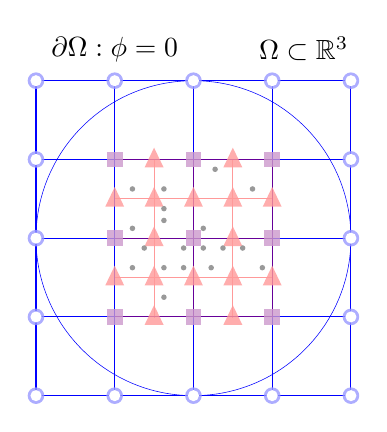
\begin{tikzpicture}[domain=-0.2:4.2,scale=1.0]
    %MG grid
    \draw[thin,color=blue,step=10mm] (0.0,0.0) grid (4,4);
    %\draw[very thin,color=gray,step=2.5mm] (0.5,-0.2) grid (3.5,1.5);
    
    %labels
    \node at (3.4,4.4) {$\Omega \subset \Re^3$};
    \node at (1,4.4) {$\partial \Omega: \phi = 0$};

    %additional grid lines MG
    %\draw[thin,color=blue] (0.5,0.0) to (0.5,4);
    %\draw[thin,color=blue] (1.5,0.0) to (1.5,4);
    %\draw[thin,color=blue] (2.5,0.0) to (2.5,4);
    %\draw[thin,color=blue] (3.5,0.0) to (3.5,4);
    
    \draw[very thin,color=blue] (2.0,2.0) circle (2);
    
    %FFT grid
    \draw[thin,color=red,step=5mm,opacity=0.4] (1.0,0.99) grid (3,3);

    %MG meshpoints
    \foreach \i in {0, 1.0, ..., 4}
    {
        \fill[blue!40,opacity=0.8] (\i,0.0) circle (3pt);
        \fill[white,opacity=1.0] (\i,0.0) circle (2pt);
    }
    \foreach \i in {0, 1.0, ..., 4}
    {
        \fill[blue!40,opacity=0.8] (\i,4.0) circle (3pt);
        \fill[white,opacity=1.0] (\i,4.0) circle (2pt);
    }
    \foreach \i in {1, ..., 3}
    {
        \fill[blue!40,opacity=0.8] (0.0,\i) circle (3pt);
        \fill[white,opacity=1.0] (0.0,\i) circle (2pt);
    }
    \foreach \i in {1, ..., 3}
    {
        \fill[blue!40,opacity=0.8] (4.0,\i) circle (3pt);
        \fill[white,opacity=1.0] (4.0,\i) circle (2pt);
    }
    
    %FFT meshpoints
    \foreach \i in {1, 1.5, ..., 3}
    {
        \fill[red!40,opacity=0.8] (\i-0.12,1.5-0.1) -- (\i,1.5+0.15) -- (\i+0.12,1.5-0.1);
    }
    \foreach \i in {1, 1.5, ..., 3}
    {
        \fill[red!40,opacity=0.8] (\i-0.12,2.5-0.1) -- (\i,2.5+0.15) -- (\i+0.12,2.5-0.1);
    }
    \foreach \j in {1.0, ..., 3.0}
    {
        \foreach \i in {1.5, ..., 2.5}
        {
            \fill[red!40,opacity=0.8] (\i-0.12,\j-0.1) -- (\i,\j+0.15) -- (\i+0.12,\j-0.1);
        }
    }
   
    %SHARED meshpoints
    \foreach \j in {1, ..., 3}
    {
        \foreach \i in {1, ..., 3}
        {
            \fill[violet!40,opacity=0.8] (\i-0.1,\j-0.1) rectangle (\i+0.1,\j+0.1);
        }
    }


    %particles
    \fill[black!40] (2.225,1.625) circle (1pt);
    \fill[black!40] (2.750,2.625) circle (1pt);
    \fill[black!40] (1.625,1.25) circle (1pt);
    
    \fill[black!40] (2.275,2.875) circle (1pt);

    \fill[black!40] (1.625,2.625) circle (1pt);
    
    \fill[black!40] (1.375,1.875) circle (1pt);

    \fill[black!40] (1.225,2.625) circle (1pt);
    \fill[black!40] (1.225,2.125) circle (1pt);
    \fill[black!40] (1.225,1.625) circle (1pt);
    
    \fill[black!40] (1.625,2.375) circle (1pt);
    \fill[black!40] (1.625,1.625) circle (1pt);
    \fill[black!40] (1.625,2.225) circle (1pt);

    \fill[black!40] (1.875,1.875) circle (1pt);
    \fill[black!40] (1.875,1.625) circle (1pt);
    
    \fill[black!40] (2.125,1.875) circle (1pt);
    \fill[black!40] (2.125,2.125) circle (1pt);

    \fill[black!40] (2.375,1.875) circle (1pt);

    \fill[black!40] (2.625,1.875) circle (1pt);
    
    \fill[black!40] (2.875,1.625) circle (1pt);

\end{tikzpicture}


        \end{minipage}
        \begin{minipage}[b]{0.45\textwidth}
        \centering
        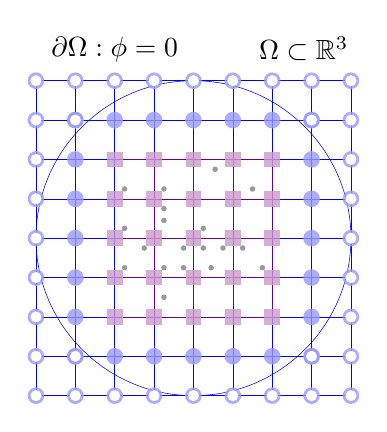
\begin{tikzpicture}[domain=-0.2:4.2,scale=1.0]
    \draw[very thin,color=blue,step=5mm] (0.0,0.0) grid (4,4);
    \draw[very thin,color=red,step=5mm,opacity=0.4] (1.0,0.99) grid (3,3);
    %\draw[very thin,color=gray,step=2.5mm] (0.5,-0.2) grid (3.5,1.5);
    
    %\filldraw[fill=gray!20,fill opacity=0.8](2,2)--(2,3)--(3,3)--(3,2)--cycle;

    %curved boundart
    %\draw (-0.2,3.55) to[out=20,in=180] node [sloped,below] {} (4.2,3.8);
    %\draw (-0.2,3.3) to[out=30,in=180] node [sloped,below] {$\Omega$} (4.2,3.8);
    
    %\coordinate [label=above:\C] (C) at (intersection of B and 1,0--1,1);
    %\fill[black,opacity=.5] C circle (2pt);
    
    \draw[very thin,color=blue] (2.0,2.0) circle (2);
  
    %labels
    \node at (3.4,4.4) {$\Omega \subset \Re^3$};
    \node at (1,4.4) {$\partial \Omega: \phi = 0$};

    \foreach \i in {0, 0.5, ..., 4}
    {
        \fill[blue!40,opacity=0.8] (\i,0.0) circle (3pt);
        \fill[white,opacity=1.0] (\i,0.0) circle (2pt);
    }
    \foreach \i in {0.5, 1.0, ..., 3.5}
    {
        \fill[blue!40,opacity=0.8] (\i,0.5) circle (3pt);
    }

    \foreach \i in {0.5, 1.0, ..., 3.5}
    {
        \fill[blue!40,opacity=0.8] (\i,3.5) circle (3pt);
    }
    \foreach \i in {0, 0.5, ..., 4}
    {
        \fill[blue!40,opacity=0.8] (\i,4.0) circle (3pt);
        \fill[white,opacity=1.0] (\i,4.0) circle (2pt);
    }
    
    \foreach \i in {1, 1.5, ..., 3}
    {
        \fill[blue!40,opacity=0.8] (0.0,\i) circle (3pt);
        \fill[white,opacity=1.0] (0.0,\i) circle (2pt);
    }
    \foreach \i in {1, 1.5, ..., 3}
    {
        \fill[blue!40,opacity=0.8] (0.5,\i) circle (3pt);
    }
    \foreach \i in {1, 1.5, ..., 3}
    {
        \fill[blue!40,opacity=0.8] (3.5,\i) circle (3pt);
    }
    \foreach \i in {1, 1.5, ..., 3}
    {
        \fill[blue!40,opacity=0.8] (4.0,\i) circle (3pt);
        \fill[white,opacity=1.0] (4.0,\i) circle (2pt);
    }
    \fill[blue!40,opacity=0.8] (3.5,3.5) circle (3pt);
    \fill[white,opacity=1.0] (3.5,3.5) circle (2pt);
    \fill[blue!40,opacity=0.8] (4.0,3.5) circle (3pt);
    \fill[white,opacity=1.0] (4.0,3.5) circle (2pt);
    
    \fill[blue!40,opacity=0.8] (0.5,3.5) circle (3pt);
    \fill[white,opacity=1.0] (0.5,3.5) circle (2pt);
    \fill[blue!40,opacity=0.8] (0.0,3.5) circle (3pt);
    \fill[white,opacity=1.0] (0.0,3.5) circle (2pt);
    
    \fill[blue!40,opacity=0.8] (3.5,0.5) circle (3pt);
    \fill[white,opacity=1.0] (3.5,0.5) circle (2pt);
    \fill[blue!40,opacity=0.8] (4.0,0.5) circle (3pt);
    \fill[white,opacity=1.0] (4.0,0.5) circle (2pt);
    
    \fill[blue!40,opacity=0.8] (0.5,0.5) circle (3pt);
    \fill[white,opacity=1.0] (0.5,0.5) circle (2pt);
    \fill[blue!40,opacity=0.8] (0.0,0.5) circle (3pt);
    \fill[white,opacity=1.0] (0.0,0.5) circle (2pt);
        
   
    \foreach \j in {1, 1.5, ..., 3}
    {
        \foreach \i in {1, 1.5, ..., 3}
        {
            \fill[violet!40,opacity=0.8] (\i-0.1,\j-0.1) rectangle (\i+0.1,\j+0.1);
        }
    }

    %\fill[violet!40,opacity=0.8] (-0.1,0.9) rectangle (0.1,1.1);
    %\fill[violet!40,opacity=0.8] (0.4,0.9) rectangle (0.6,1.1);
    %\fill[violet!40,opacity=0.8] (0.9,0.9) rectangle (1.1,1.1);

    %particles
    \fill[black!40] (2.225,1.625) circle (1pt);
    \fill[black!40] (2.750,2.625) circle (1pt);
    \fill[black!40] (1.625,1.25) circle (1pt);
    
    \fill[black!40] (2.275,2.875) circle (1pt);

    \fill[black!40] (1.625,2.625) circle (1pt);
    
    \fill[black!40] (1.375,1.875) circle (1pt);

    \fill[black!40] (1.125,2.625) circle (1pt);
    \fill[black!40] (1.125,2.125) circle (1pt);
    \fill[black!40] (1.125,1.625) circle (1pt);
    
    \fill[black!40] (1.625,2.375) circle (1pt);
    \fill[black!40] (1.625,1.625) circle (1pt);
    \fill[black!40] (1.625,2.225) circle (1pt);

    \fill[black!40] (1.875,1.875) circle (1pt);
    \fill[black!40] (1.875,1.625) circle (1pt);
    
    \fill[black!40] (2.125,1.875) circle (1pt);
    \fill[black!40] (2.125,2.125) circle (1pt);

    \fill[black!40] (2.375,1.875) circle (1pt);

    \fill[black!40] (2.625,1.875) circle (1pt);
    
    \fill[black!40] (2.875,1.625) circle (1pt);

\end{tikzpicture}


        \end{minipage} 

    \end{frame}


	\begin{frame}
		\frametitle{Implementation (2/4)}
		\framesubtitle{Integration in \opal I: Class Hierarchy}

		\begin{center}
		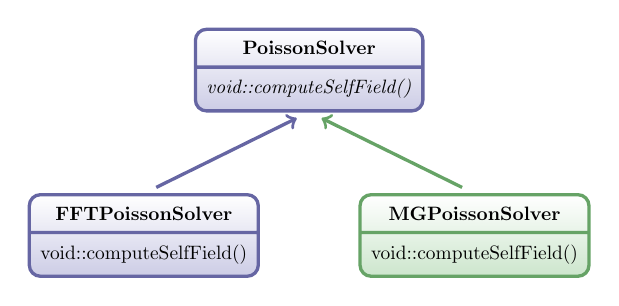
\begin{tikzpicture}[scale=0.7, transform shape, grow=down, level 1/.style={sibling distance=6cm,level distance=3cm},edge from parent/.style={very thick,draw=blue!40!black!60,shorten >=5pt, shorten <=5pt},edge from parent path={(\tikzparentnode.south) -- (\tikzchildnode.north)},every node/.style={text ragged, inner sep=2mm}]

			\tikzstyle{class} = [rectangle, rounded corners, shade, top color=white,bottom color=blue!50!black!20, draw=blue!40!black!60, very thick];
			\tikzstyle{newclass} = [rectangle, rounded corners, shade, top color=white,bottom color=green!50!black!20, draw=green!40!black!60, very thick];

			\node[class] [rectangle split, rectangle split, rectangle split parts=2, text ragged] {
			    \textbf{PoissonSolver}
			    \nodepart{second} 
			    	\textit{void::computeSelfField()}
			}
			    child {
			        node[class] [rectangle split, rectangle split parts=2, text ragged] {
			            \textbf{FFTPoissonSolver}
			            \nodepart{second} 
				      void::computeSelfField() 
			        }
		        edge from parent [<-]
		    }
			    child {
			    	node[newclass] [rectangle split, rectangle split parts=2, text ragged] {
				    \textbf{MGPoissonSolver}
				    \nodepart{second} 
				      void::computeSelfField() 
				}
		        edge from parent [<-, draw=green!40!black!60]
		   };
		\end{tikzpicture}
		\end{center}

	\end{frame}

	\begin{frame}
		\frametitle{Implementation (1/3)}
		\framesubtitle{Class Diagram}

		\begin{center}
		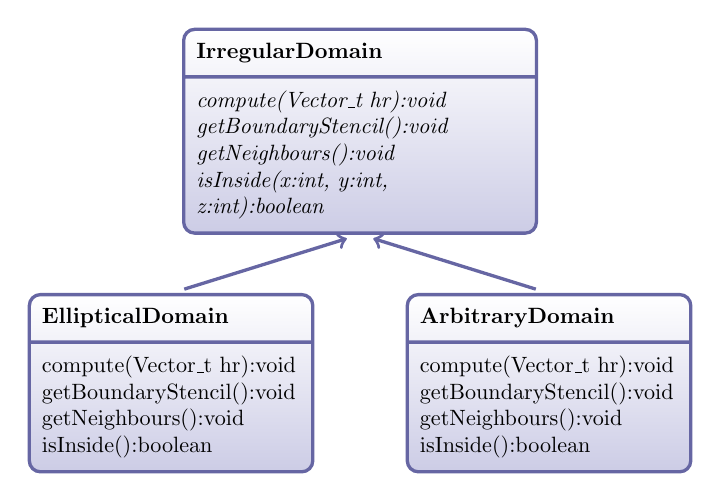
\begin{tikzpicture}[scale=0.8, transform shape, grow=down, level 1/.style={sibling distance=6cm,level distance=4cm},edge from parent/.style={very thick,draw=blue!40!black!60,shorten >=5pt, shorten <=5pt},edge from parent path={(\tikzparentnode.south) -- (\tikzchildnode.north)},every node/.style={text ragged, inner sep=2mm}]

\tikzstyle{class} = [rectangle, rounded corners, shade, top color=white,bottom color=blue!50!black!20, draw=blue!40!black!60, very thick];

\node[class] [rectangle split, rectangle split parts=2, text width=5.2cm] {
    \textbf{IrregularDomain}
    \nodepart{second} 
    	\textit{compute(Vector\_t hr):void} \\
	\textit{getBoundaryStencil():void} \\
	\textit{getNeighbours():void} \\
	\textit{isInside(x:int, y:int, z:int):boolean}
    }
    child {
        node[class] [rectangle split, rectangle split parts=2, text width=4.1cm] {
            \textbf{EllipticalDomain}
            \nodepart{second} 
	      compute(Vector\_t hr):void \\
	      getBoundaryStencil():void \\
	      getNeighbours():void \\
	      isInside():boolean
        }
        edge from parent [<-]
    }
    child {
    	node[class] [rectangle split, rectangle split parts=2, text width=4.1cm] {
	    \textbf{ArbitraryDomain}
	    \nodepart{second} 
	      compute(Vector\_t hr):void \\
	      getBoundaryStencil():void \\
	      getNeighbours():void \\
	      isInside():boolean
	}
        edge from parent [<-]
   };
\end{tikzpicture}
\end{center}


	\end{frame}
	
    \begin{frame}
        \frametitle{Implementation (3/3)}
        \framesubtitle{Interface between \textsc{IPPL} and \textsc{Epetra}}

        \begin{block}{\textsc{IPPL} to \textsc{Epetra} Map}
        \begin{algorithmic}[1]
            \STATE \textbf{procedure} IPPLToMap3D(localidx)

            \STATE idx $\leftarrow$ 0

            \FORALL{localidx.$x$}
                \FORALL{localidx.$y$}
                    \FORALL{localidx.$z$}
                        \STATE MyGlobalElements[idx] $\leftarrow$ bp$\rightarrow$getIdx($x$,$y$,$z$)
                        \STATE idx $\leftarrow$ $\text{idx} + 1$
                    \ENDFOR
                \ENDFOR
            \ENDFOR
            
            \RETURN \textbf{new} Epetra\_Map(-1, NumMyElements, \&MyGlobalElements[0], 0, Comm)
            \STATE \textbf{end procedure}
          \end{algorithmic}
        \end{block}

    \end{frame}
    
    \begin{frame}{Implementation}
		\framesubtitle{Importing geometries in \opal}
    
		\begin{columns}
		\begin{column}{6.6cm}
        \begin{center}
        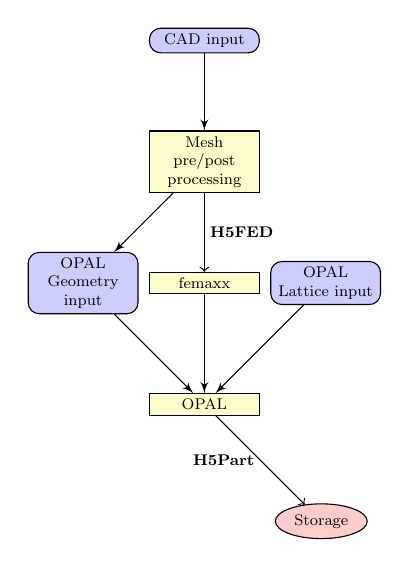
\begin{tikzpicture}[scale=0.7,transform shape,node distance=2.2cm] \footnotesize
            \node [pblock] (CAD) {CAD input};
            \node [progblock, below of= CAD] (HERONION) {Mesh pre/post processing};
            \node [progblock,below of= HERONION] (FEMAXX) {femaxx};
            \node [pblock,left of= FEMAXX] (OPALGEO) {OPAL Geometry input};
            \node [pblock,right of= FEMAXX] (OPALLAT) {OPAL Lattice input};
            \node [progblock, below of=FEMAXX] (OPAL) {OPAL};
            \node [cloud,below right of= OPAL](DISK){Storage};

            % Draw edges
            \path [line] (CAD) -> (HERONION);
            \path [line,->] (HERONION) edge   node[right] {\bf H5FED} (FEMAXX);
            \path [line] (FEMAXX) -> (OPAL);
            \path [line,->] (OPAL) edge node[left] {\bf H5Part}   (DISK);
            \path [line] (HERONION) -> (OPALGEO);

            \path [line] (OPALLAT) -> (OPAL);
            \path [line] (OPALGEO) -> (OPAL);
        \end{tikzpicture}\\
        \end{center}
		\end{column}
		\begin{column}{5cm}	
			\begin{center}
			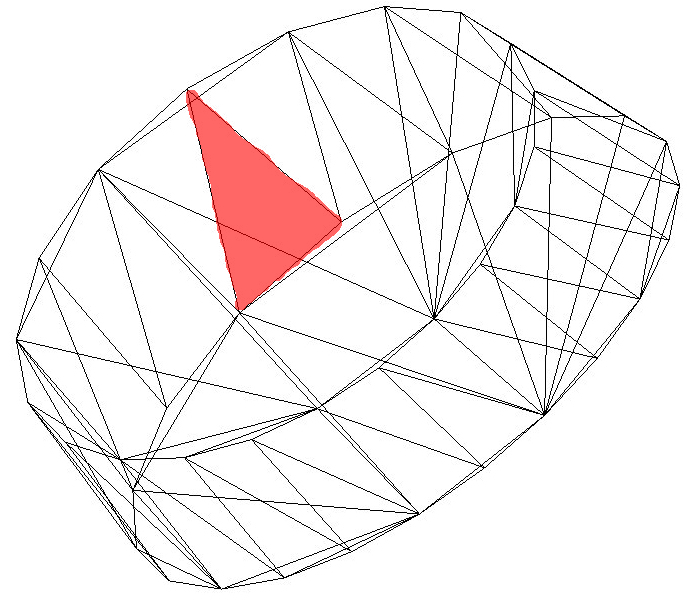
\includegraphics[width=1.0\textwidth]{cylinder-col.jpg} %problem? 

            \vspace{0.2cm}

            Efficient Intersection of Grid-Lines with Triangular Surface Mesh (T. Moeller, B. Trumbore, 1997)
			\end{center}
		\end{column}
		\end{columns}

    \end{frame}
	
    \begin{frame}
        \frametitle{Implementation (2/2)}
        \framesubtitle{Setup Phase}

        \begin{columns}
        \begin{column}{6.6cm}
        \begin{itemize}
            \item extended \textsc{Heronion} to dump H5Fed surface mesh
            \item \opal imports H5Fed files (serial): $m$ triangles and $v$ vertices
            \item efficient intersection of grid-lines with triangular surface mesh (T. Moeller and B. Trumbore (1997)): 
                \begin{itemize}
                    \item arbitrary domain: $O(m(n_x+n_y+local_z))$ 
                    \item elliptic domain: $O(n_x + n_y)$
                \end{itemize}
            \item building index table
                \begin{itemize}
                    \item arbitrary domain: $O(n_x n_y local_z)$
                    \item elliptic domain: $O(n_x n_y)$
                \end{itemize}
        \end{itemize}
        \end{column}
        \begin{column}{4cm}	
            \begin{center}
            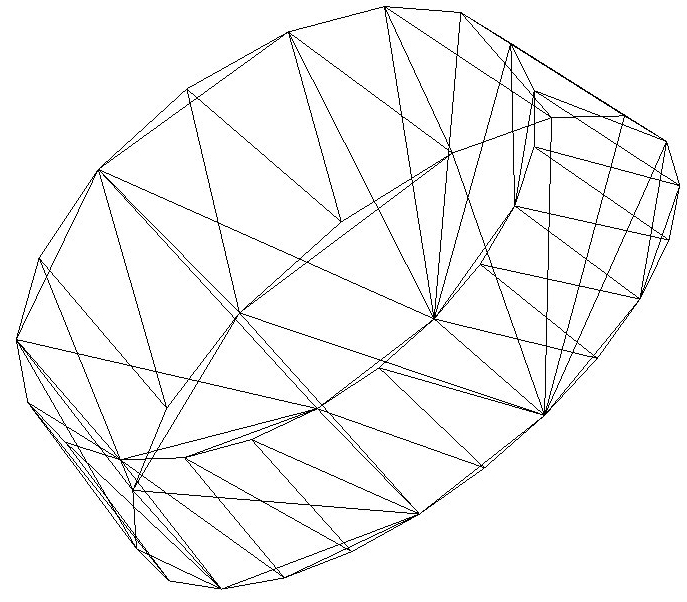
\includegraphics[width=1.0\textwidth]{cylinder.jpg}
            \end{center}
        \end{column}
        \end{columns}

    \end{frame}

	\begin{frame}
		\frametitle{SW: non-symmetries}

		\begin{center}
		    \begin{tikzpicture}[domain=-0.2:4.2,scale=1.4]
    \draw[very thin,color=gray,step=10mm] (-0.2,-0.2) grid (4.2,4.2);
    
    %curved boundart
    \draw (0,0) to[out=90,in=180] node [sloped,below] {} (2,4);
  
    \node at (4.6,4.2) {$\Omega \subset \Re^3$};
    \node at (-0.8,2.5) {$\partial \Omega: \phi = 0$};

    \draw[thick,color=red] (0.18,2) to node[above] {$G_w$}(1,2);
    \draw[thick,color=red] (0.48,3) to node[below] {$H_w$}(1,3);

    \fill[blue!60,opacity=0.5] (1,2) node[right] {$G$} circle (2pt);
    \fill[blue!60,opacity=0.5] (1,3) node[right] {$H$} circle (2pt);

\end{tikzpicture}

		\end{center}

	\end{frame}
	
	\begin{frame}
		\frametitle{Grid Operators}
		\framesubtitle{AMG: smoothed aggregation}

		%TODO: finish

		Operate on directly on (linear sparse) algebraic equations:

		\[
			\sum_j a_{ij}^h x_j^h = b_i^h
		\]

		\begin{itemize}
			\item replace "grid" with "variables"
			%\item AMG fixes smoother and adjusts coarsening (GMG inverse)
			\item coarse level equations are generated without the use of any geometry
			\item no coarse level grids have to be generated or stored
			\item good preconditioner: works on all error components (in contrast to level-one preconditioner)
		\end{itemize}

		\vspace{0.2cm}
		SA restrict operator:

		\[
			I_H^h = (I_h - \omega D_h^{-1} A_h^f) \hat{I}_H^h
		\]

		%generate operator dependet interpolation and Galerkin operator can be derived directly from the underlying matrices, without any reference to the actual grids.
	
  	\end{frame}

    	\begin{frame}
		\frametitle{Multigrid Theory (1/2)}
		\framesubtitle{Motivation}

		\begin{block}{Important Observations}
			\begin{itemize}
				\item Some classical iterative methods (i.e. Gauss Seidel) have a smoothing effect on the error of any approximation for discrete elliptic problems.
				\vspace{0.2cm}
				\item A smooth error can be well approximated on a coarse grid. This coarse grid has considerably fewer grid points and is therefore cheaper to solve.
			\end{itemize}
		\end{block}

		\vspace{0.4cm}

		From this two observations a Two-Grid can be deduced:

		\begin{enumerate}
			\item apply smoother
			\item restrict to a grid with considerably fewer grid points (coarse)
			\item solve
			\item interpolate back to the fine grid
			\item compute a new approximation
		\end{enumerate}

	\end{frame}
    	
	\begin{frame}
		\frametitle{Multigrid Theory (2/2)}
		\framesubtitle{The Two-Grid: Smoothed Coarse Grid Correction}

		The discretized system is solved by a Two-Grid:

		\[
			A\mathbf{x} = \mathbf{b}
		\]
		\[
			e_h^m = x_h - x_h^m\text{, } r_h^m = b_h - A_hx_h^m
		\]
		\[
			r_h^m = A_h e_h^m
		\]

		\vspace{0.1cm}

		\begin{center}
		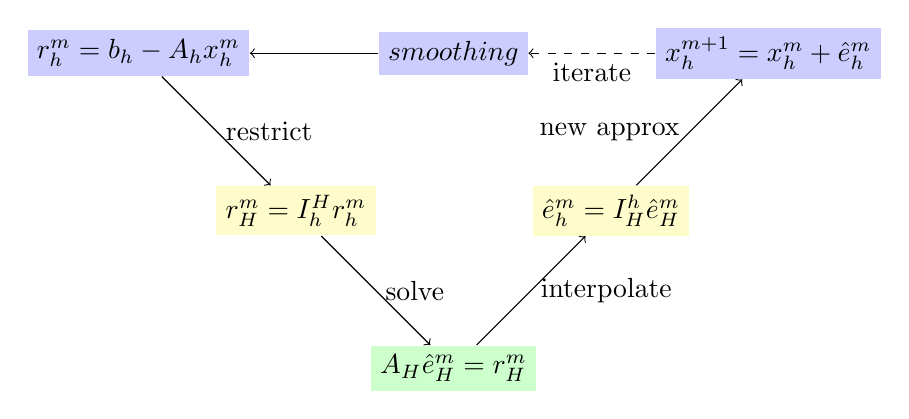
\begin{tikzpicture}[scale=1,transform shape,node distance=2cm]	
            		\node[fill=blue!20] (res)
            		{$ r_h^m = b_h - A_h x_h^m $};
			\node[right of=res] (dummy6) {};
            		\node[fill=blue!20, right of=dummy6] (smooth)
            		{$ smoothing $};
			\node[below of=res] (dummy1) {};
            		\node[fill=yellow!20, right of=dummy1] (restrict)
            		{$ r_H^m = I_h^H r_h^m$};
			\node[below of=restrict] (dummy2) {};
            		\node[fill=green!20, right of=dummy2] (solve)
            		{$ A_H \hat{e}_H^m = r_H^m $};
			\node[right of=solve] (dummy3) {};
            		\node[fill=yellow!20, above of=dummy3] (interpolate)
            		{$ \hat{e}_h^m = I_H^h \hat{e}_H^m $};
			\node[right of=interpolate] (dummy4) {};
            		\node[fill=blue!20, above of=dummy4] (newapprox)
			{$ x_h^{m+1} = x_h^m + \hat{e}_h^m $};

        		\path[->] (res) edge node[right] {restrict} (restrict);
        		\path[->] (restrict) edge node[right] {solve} (solve);
        		\path[->] (solve) edge node[right] {interpolate} (interpolate);
        		\path[->] (interpolate) edge node[left] {new approx} (newapprox);
        		\path[->] (smooth) edge (res);
        		\path[->,dashed] (newapprox) edge node[below] {iterate} (smooth);
		\end{tikzpicture}
		\end{center}

	\end{frame}

	\begin{frame}
		\frametitle{Grid Operators}
		\framesubtitle{Geometric Multigrid}

		\begin{columns}
		\begin{column}{4.5cm}
		\textbf{restriction} \\
		\vspace{0.4cm}
		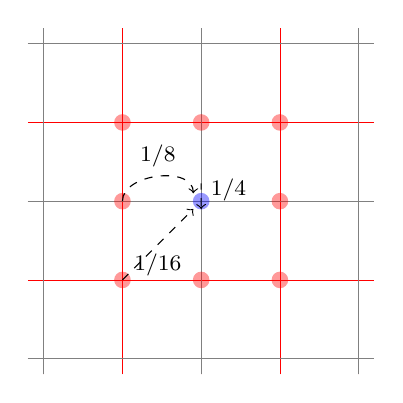
\begin{tikzpicture}[scale=1.0,transform shape,node distance=1cm]	
			\draw[very thin,color=red,step=1cm] (-0.2,-0.2) grid (4.2,4.2);
			\draw[very thin,color=gray,step=2cm] (-0.2,-0.2) grid (4.2,4.2);
			
			%\draw[very thin,color=gray,step=2cm] (5,-0.2) grid (9.2,4.2);
    
			\fill[color=blue,opacity=0.4] (2.0,2.0) circle (3pt);
			\fill[color=red,opacity=0.4] (1.0,2.0) circle (3pt);
			\fill[color=red,opacity=0.4] (1.0,1.0) circle (3pt);
			\fill[color=red,opacity=0.4] (2.0,1.0) circle (3pt);
			\fill[color=red,opacity=0.4] (3.0,2.0) circle (3pt);
			\fill[color=red,opacity=0.4] (2.0,3.0) circle (3pt);
			\fill[color=red,opacity=0.4] (3.0,3.0) circle (3pt);
			\fill[color=red,opacity=0.4] (1.0,3.0) circle (3pt);
			\fill[color=red,opacity=0.4] (3.0,1.0) circle (3pt);
			
    			\path[style=dashed, ->] (1.0,2.0) edge [out=90, in=90] node[above] {\footnotesize{$1/8$}} (1.9,2.1);
    			\path[style=dashed, ->] (1.0,1.0) edge node[below] {\footnotesize{$1/16$}} (1.9,1.9);
    			\path[style=dashed, ->] (2.0,2.2) edge [out=90, in=91] node[right] {\footnotesize{$1/4$}} (2.0,1.9);

		\end{tikzpicture}
		\end{column}

		\begin{column}{4.5cm}
		\textbf{bilinear interpolation} \\
		\vspace{0.4cm}
		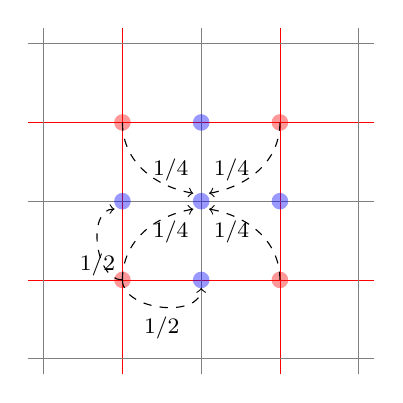
\begin{tikzpicture}[scale=1.0 ,transform shape,node distance=1cm]	
			\draw[very thin,color=red,step=1cm] (-0.2,-0.2) grid (4.2,4.2);
			\draw[very thin,color=gray,step=2cm] (-0.2,-0.2) grid (4.2,4.2);
			
			%\draw[very thin,color=gray,step=2cm] (5,-0.2) grid (9.2,4.2);
    
			\fill[color=blue,opacity=0.4] (2.0,2.0) circle (3pt);
			\fill[color=blue,opacity=0.4] (1.0,2.0) circle (3pt);
			\fill[color=red,opacity=0.4] (1.0,1.0) circle (3pt);
			\fill[color=blue,opacity=0.4] (2.0,1.0) circle (3pt);
			\fill[color=blue,opacity=0.4] (3.0,2.0) circle (3pt);
			\fill[color=blue,opacity=0.4] (2.0,3.0) circle (3pt);
			\fill[color=red,opacity=0.4] (3.0,3.0) circle (3pt);
			\fill[color=red,opacity=0.4] (1.0,3.0) circle (3pt);
			\fill[color=red,opacity=0.4] (3.0,1.0) circle (3pt);
			
    			
			\path[style=dashed, ->] (3.0,3.0) edge [out=-90, in=10] node[left] {\footnotesize{$1/4$}} (2.1,2.1);
    			\path[style=dashed, ->] (1.0,3.0) edge [out=-90, in=170] node[right] {\footnotesize{$1/4$}} (1.9,2.1);
    			\path[style=dashed, ->] (3.0,1.0) edge [out=90, in=-10] node[left] {\footnotesize{$1/4$}} (2.1,1.9);
    			\path[style=dashed, ->] (1.0,1.0) edge [out=90, in=-170] node[right] {\footnotesize{$1/4$}} (1.9,1.9);

    			\path[style=dashed, ->] (1.0,1.0) edge [out=-90, in=-90] node[below] {\footnotesize{$1/2$}} (2.0,0.9);
    			\path[style=dashed, ->] (1.0,1.0) edge [out=180, in=180] node[below] {\footnotesize{$1/2$}} (0.9,1.9);
		\end{tikzpicture}
		\end{column}
		\end{columns}

	\end{frame}
	

	\begin{frame}
		\frametitle{Multigrid}
		\framesubtitle{from Two-Grid to Multigrid}

		%v -> V / W (etc)
		\begin{center}
		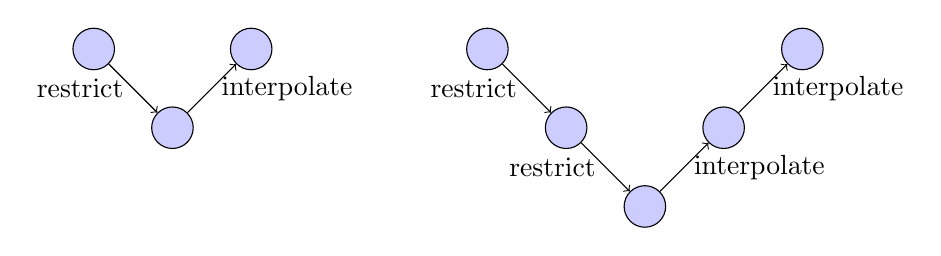
\begin{tikzpicture}[scale=1,transform shape,node distance=1cm]	
			\tikzstyle{circ} = [circle, draw, thin, fill=blue!20, minimum height=1.5em]

			%v
			\node[circ] (v1) {};
			\node[right of=v1] (dummy1) {};
			\node[circ,below of=dummy1] (v2) {};
			\node[circ,right of=dummy1] (v3) {};
        		\path[->] (v1) edge node[left] {restrict} (v2);
        		\path[->] (v2) edge node[right] {interpolate} (v3);
			
			%V
			\node[right of=v3] (DD) {};
			\node[right of=DD] (D) {};
			\node[circ,right of=D] (V1) {};
			\node[right of=V1] (Dummy1) {};
			\node[circ,below of=Dummy1] (V2) {};
			\node[right of=V2] (Dummy2) {};
			\node[circ,below of=Dummy2] (V3) {};
			\node[circ,right of=Dummy2] (V4) {};
			\node[above of=V4] (Dummy3) {};
			\node[circ,right of=Dummy3] (V5) {};
			
        		\path[->] (V1) edge node[left] {restrict} (V2);
        		\path[->] (V2) edge node[left] {restrict} (V3);
        		\path[->] (V3) edge node[right] {interpolate} (V4);
        		\path[->] (V4) edge node[right] {interpolate} (V5);
        		
		\end{tikzpicture}
		\end{center}

		\vspace{0.3cm}

		Depending on how the recursion is coded, some variants of the V-cycle can be produced.

		\begin{itemize}
			\item grid-independence convergence 
			\item iterative solver: reuse information
			\item $\mathcal{O}(n)$ algorithm
		\end{itemize}
			
		\textbf{Anisotropy} is handled in the discretized problem

	\end{frame}
	
    \begin{frame}
        \frametitle{Multigrid Algorithm}

        %\begin{algorithm}
        %\caption{Multigrid V-cycle Algorithm}
        \begin{block}{Mutligrid V-Cycle Algorithm}
        \begin{algorithmic}[1]
            \STATE \textbf{procedure} MultiGridSolve($A_l$, $b_l$, $x_l$, $l$)

            \IF{$l$ = maxLevel-1}
                \STATE DirectSolve $A_l \mathbf{x}_l = \mathbf{b}_l$
            \ELSE
                \STATE $\mathbf{x}_l$ $\leftarrow$ $S^{pre}_l$($A_l$, $\mathbf{b}_l$, $0$)
                \STATE $\mathbf{r}_l$ $\leftarrow$ $\mathbf{b}_l$ - $A_l \mathbf{x}_l$ \COMMENT{calculate residual}
                \STATE $\mathbf{b}_{l+1}$ $\leftarrow$ $R_l \mathbf{r}_l$ \COMMENT{Restriction}
                \STATE $\mathbf{v}_{l+1}$ $\leftarrow$ $\mathbf{0}$
                \STATE MultiGridSolve($A_{l+1}$, $\mathbf{b}_{l+1}$, $\mathbf{v}_{l+1}$, $l+1$)
                \STATE $\mathbf{x}_l$ $\leftarrow$ $\mathbf{x}_l$ + $P_l \mathbf{v}_{l+1}$ \COMMENT{coarse grid correction}
                \STATE $\mathbf{x}_l$ $\leftarrow$ $S^{post}_l$($A_l$, $\mathbf{b}_l$, $\mathbf{x}_l$)
            \ENDIF
            \STATE \textbf{end procedure}
        \end{algorithmic}
        %\end{algorithm}
        \end{block}

    \end{frame}

    \begin{frame}
        \frametitle{Smoothed Aggregation: The Grid Transfer Operator}

        \begin{columns}
        \begin{column}{6.7cm}
            \begin{enumerate}
                \item discretization matrix $A_l$ is converted into a graph $G_l$
                \item assign each {\color{blue!60}vertex} of $G_l$ is assigned to one {\color{red!60}aggregate} % of the disjoint aggregate set where each aggregate represents a coarse grid vertex
                \item the tentative prolongation operator matrix is formed 
                \begin{itemize}
                    \item matrix rows correspond to vertices
                    \item matrix columns to aggregates
                    \[
                        p_{i,j} = \begin{cases} 1 & \text{if } i^{th} \text{ vertex in } j^{th} \text{ aggregate} \\ 
                                        0 & \text{otherwise}
                              \end{cases}
                    \]
                \end{itemize}
                \item improve robustness by smoothing the tentative prolongation operator

            \end{enumerate}
        \end{column}

        \begin{column}{4cm}
            \begin{center}
                %%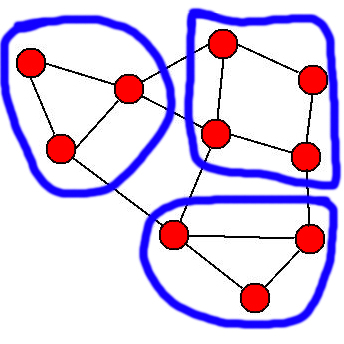
\includegraphics[width=1.0\textwidth]{aggregation.jpg} 
                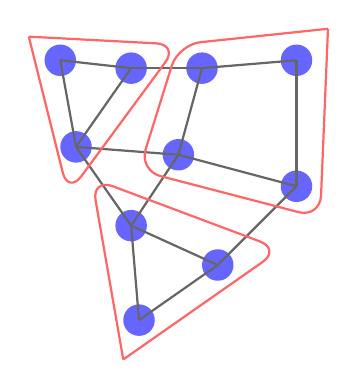
\begin{tikzpicture}
                    \colorlet{CRSTENCIL}{blue!60!white}
                    \colorlet{ML}{green!75!black!60!white}
                    \colorlet{CG}{red!60!white}
                    \colorlet{RECALCMAP}{black!60}

                    \node [coordinate] at (0,0) (N1) {};
                    \fill[color=blue!60] (N1) circle (0.2);
                    \node [coordinate] at (1,0.7) (N2) {};
                    \fill[color=blue!60] (N2) circle (0.2);
                    \node [coordinate] at (-0.10,1.2) (N3) {};
                    \fill[color=blue!60] (N3) circle (0.2);

                    \node [coordinate] at (-0.80,2.2) (N4) {};
                    \fill[color=blue!60] (N4) circle (0.2);
                    \node [coordinate] at (-0.10,3.2) (N5) {};
                    \fill[color=blue!60] (N5) circle (0.2);
                    \node [coordinate] at (-1.00,3.3) (N6) {};
                    \fill[color=blue!60] (N6) circle (0.2);

                    \node [coordinate] at (2,1.7) (N7) {};
                    \fill[color=blue!60] (N7) circle (0.2);
                    \node [coordinate] at (0.5,2.1) (N8) {};
                    \fill[color=blue!60] (N8) circle (0.2);
                    \node [coordinate] at (2,3.3) (N9) {};
                    \fill[color=blue!60] (N9) circle (0.2);
                    \node [coordinate] at (0.8,3.2) (N10) {};
                    \fill[color=blue!60] (N10) circle (0.2);

                    \path[-,thick,color=black!60]<1-> (N1) edge (N2);
                    \path[-,thick,color=black!60]<1-> (N1) edge (N3);
                    \path[-,thick,color=black!60]<1-> (N2) edge (N3);
                    
                    \path[-,thick,color=black!60]<1-> (N2) edge (N7);
                    \path[-,thick,color=black!60]<1-> (N3) edge (N8);
                    
                    \path[-,thick,color=black!60]<1-> (N4) edge (N5);
                    \path[-,thick,color=black!60]<1-> (N4) edge (N6);
                    \path[-,thick,color=black!60]<1-> (N5) edge (N6);
                    
                    \path[-,thick,color=black!60]<1-> (N3) edge (N4);
                    \path[-,thick,color=black!60]<1-> (N8) edge (N4);

                    \path[-,thick,color=black!60]<1-> (N7) edge (N8);
                    \path[-,thick,color=black!60]<1-> (N7) edge (N9);
                    \path[-,thick,color=black!60]<1-> (N8) edge (N10);
                    \path[-,thick,color=black!60]<1-> (N9) edge (N10);
                    
                    \path[-,thick,color=black!60]<1-> (N5) edge (N10);

                    \draw[thick,rounded corners=8pt,color=red!60] (-0.2,-0.5) -- (1.8,0.9) -- (-0.6,1.8) -- (-0.2,-0.5);
                    \draw[thick,rounded corners=8pt,color=red!60] (2.4,3.7) -- (0.5, 3.5) -- (0.0,1.9) -- (2.3,1.3) -- (2.4,3.7);
                    \draw[thick,rounded corners=8pt,color=red!60] (-1.4,3.6) -- (-0.9,1.6) -- (0.5,3.5) -- (-1.4,3.6);


                \end{tikzpicture}
                \scriptsize{\\clustering vertices into aggregates}
            \end{center}
        \end{column}
        \end{columns}

    \end{frame}
	
    \begin{frame}
		\frametitle{Discretization: Irregular Domains (1/2)}
		\framesubtitle{$O(h)$ Approach}

		The key idea of this approach is to only consider grid points inside the domain neglecting the distance to the domain boundary:
		\[
			(h_w^{-1}+h_s^{-1}+h_e^{-1}+h_n^{-1})u_p - h_n^{-1} u_n - h_w^{-1} u_w - h_s^{-1} u_s - h_e^{-1} \underbrace{u_e}_{=0} = f_p
		\]

		\vspace{0.5cm}
	
		\begin{alertblock}{Properties}
		\begin{itemize}
			\item the resulting discretization matrix is symmetric
			\item $O(h)$ accurate
		\end{itemize}
		\end{alertblock}

	\end{frame}
	
	\begin{frame}
		\frametitle{Discretization: Irregular Domains (2/2)}
		\framesubtitle{Shortley-Weller approximation}
	
		\begin{columns}
		\begin{column}{4cm}	
			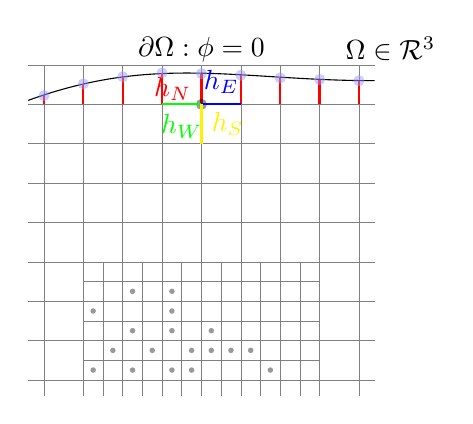
\begin{tikzpicture}[domain=-0.2:4.2,scale=1.0]
    \draw[very thin,color=gray,step=5mm] (-0.2,-0.2) grid (4.2,4);
    \draw[very thin,color=gray,step=2.5mm] (0.5,-0.2) grid (3.5,1.5);
    
    %\filldraw[fill=gray!20,fill opacity=0.8](2,2)--(2,3)--(3,3)--(3,2)--cycle;

    %curved boundart
    \draw (-0.2,3.55) to[out=20,in=180] node [sloped,below] {} (4.2,3.8);
    %\draw (-0.2,3.3) to[out=30,in=180] node [sloped,below] {$\Omega$} (4.2,3.8);
    
    %\coordinate [label=above:\C] (C) at (intersection of B and 1,0--1,1);
    %\fill[black,opacity=.5] C circle (2pt);
  
    %labels
    \node at (4.4,4.2) {$\Omega \in \mathcal{R}^3$};
    \node at (2,4.2) {$\partial \Omega: \phi = 0$};

    %interpolation lines
    \draw[thick,color=red] (0.0,3.5) to (0.0,3.61);
    \draw[thick,color=red] (0.5,3.5) to (0.5,3.76);
    \draw[thick,color=red] (1.0,3.5) to (1.0,3.85);
    \draw[thick,color=red] (1.5,3.5) to (1.5,3.90);
    \draw[thick,color=red] (2.0,3.5) to node[left] {$h_N$}(2.0,3.89);
    \draw[thick,color=red] (2.5,3.5) to (2.5,3.87);
    \draw[thick,color=red] (3.0,3.5) to (3.0,3.835);
    \draw[thick,color=red] (3.5,3.5) to (3.5,3.815);
    \draw[thick,color=red] (4.0,3.5) to (4.0,3.8);

    %on example interpol-point
    \fill[color=black,opacity=0.4] (2.0,3.5) circle (2pt);
    \draw[thick,color=green] (2.0,3.5) to node[below] {$h_W$} (1.5,3.5);
    \draw[thick,color=blue] (2.0,3.5) to node[above] {$h_E$} (2.5,3.5);
    \draw[thick,color=yellow] (2.0,3.5) to node[right] {$h_S$} (2.0,3.0);
    %\node at (2.2,3.7) {$h_{E}$};
    %\node at (1.7,3.7) {$h_{W}$};
    %\node at (2.2,3.2) {$h_{S}$};
    %\node at (2.2,3.2) {$h_{N}$};


    %short notice: dont use intersect
    \fill[blue!40,opacity=0.5] (0,3.61) circle (2pt);
    \fill[blue!40,opacity=0.5] (0.5,3.76) circle (2pt);
    \fill[blue!40,opacity=0.5] (1,3.85) circle (2pt);
    \fill[blue!40,opacity=0.5] (1.5,3.9) circle (2pt);
    \fill[blue!40,opacity=0.5] (2,3.89) circle (2pt);
    \fill[blue!40,opacity=0.5] (2.5,3.87) circle (2pt);
    \fill[blue!40,opacity=0.5] (3,3.835) circle (2pt);
    \fill[blue!40,opacity=0.5] (3.5,3.815) circle (2pt);
    \fill[blue!40,opacity=0.5] (4,3.8) circle (2pt);

    %particles
    \fill[black!40] (0.625,0.125) circle (1pt);
    \fill[black!40] (0.625,0.875) circle (1pt);
    
    \fill[black!40] (0.875,0.375) circle (1pt);

    \fill[black!40] (1.625,1.125) circle (1pt);
    
    \fill[black!40] (1.375,0.375) circle (1pt);

    \fill[black!40] (1.125,1.125) circle (1pt);
    \fill[black!40] (1.125,0.625) circle (1pt);
    \fill[black!40] (1.125,0.125) circle (1pt);
    
    \fill[black!40] (1.625,0.875) circle (1pt);
    \fill[black!40] (1.625,0.125) circle (1pt);
    \fill[black!40] (1.625,0.625) circle (1pt);

    \fill[black!40] (1.875,0.375) circle (1pt);
    \fill[black!40] (1.875,0.125) circle (1pt);
    
    \fill[black!40] (2.125,0.375) circle (1pt);
    \fill[black!40] (2.125,0.625) circle (1pt);

    \fill[black!40] (2.375,0.375) circle (1pt);

    \fill[black!40] (2.625,0.375) circle (1pt);
    
    \fill[black!40] (2.875,0.125) circle (1pt);

\end{tikzpicture}

		\end{column}
		\begin{column}{6.5cm}	
		\small{	
			\[
				2 \begin{bmatrix}
				& \frac{b}{h_N (h_N + h_S)} & \\ 
                \frac{a}{h_W (h_W + h_E)} & -\frac{a}{h_w h_E} -\frac{b}{h_S h_N} & \frac{a}{h_E (h_W + h_E)} \\
                & \frac{b}{h_S (h_N + h_S)} & \\
                \end{bmatrix}_h
			\] 
		}
		\end{column}
		\end{columns}
		
		\begin{alertblock}{Properties}
		\begin{itemize}
			\item the resulting discretization matrix is non-symmetric for boundary points
			\item $O(h^2)$ accurate
		\end{itemize}
		\end{alertblock}

	\end{frame}

%	\appendix
%	\begin{frame}
%	  \frametitle<presentation>{References}
%	  \begin{thebibliography}{10}
%	  \beamertemplatearticlebibitems
%	
%	  \bibitem{BAISU2005}
%	    Z.\ Bai. \scriptsize{AND} \normalsize{Y.\ Su.}
%	    \newblock {\em SOAR: A Second-Order Arnoldi Method for the Solution of the Quadratic Eigenvalue Problem}.
%	    \newblock SIAM J. Matrix Anal. Appl., 2005.
%
%	  \bibitem{PRESVAR}
%	    \textbf{L.\ Lee.}, L.\ Ge., Z.\ Li., C.\ Ng., K.\ Ko., B.\ Liao., Z.\ Bai., D.\ Gao., W.\ Gao., C.\ Yang., P.\ Husbands., E.G.\ Ng.
%	    \newblock{\em Solving Nonlinear Eigenproblems in Acclerator Cavity Design}.
%	    \newblock SIAM Annual Meeting, MS 44 and MS 56: Nonlinear Eigenvalue Problems, 2005
%	    
%	  \end{thebibliography}
%	\end{frame}

\end{document}
